
\begin{frame}
\frametitle{LDA: an optimal binary linear classifier}
\begin{columns}
\begin{column}{.5\linewidth}
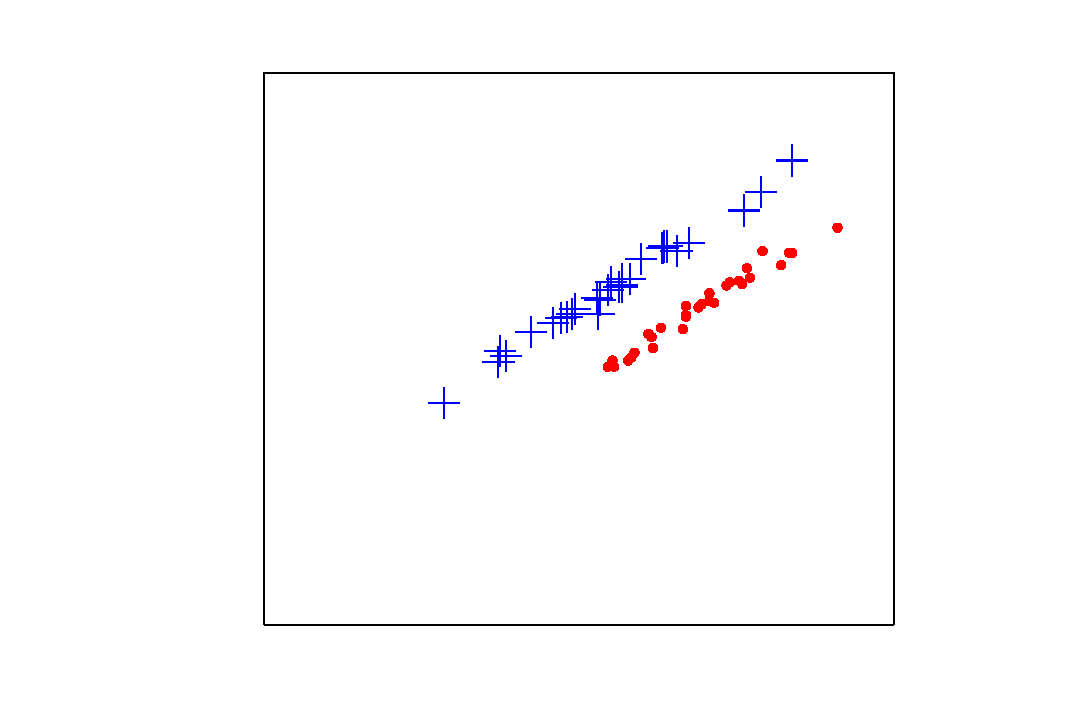
\includegraphics[width=\textwidth]{figures/dataNoProjection.pdf} 
\end{column}
\begin{column}{.6\linewidth}
\begin{itemize}
\item Classify data $\vLeakVec$ into 2 classes $\sensVarSet = \{\sensVarValue{1}, \sensVarValue{2}\}$
\pause
\item Generative model: $\pdf_{\given{\vaLeakVec}{\sensRandVar = \sensVarValue{j}}}(\vLeakVec)$, $\pdf_{\sensRandVar}(\sensVarValue{j})$ and $\pdf_{\vaLeakVec}(\vLeakVec)$
\pause
\item Posterior probabilities (via Bayes' theorem), then classify through the \emph{log-likelihood ratio}: $a = \log\left[\frac{\prob(\given{\sensVarValue{1}}{\vLeakVec})}{\prob(\given{\sensVarValue{2}}{\vLeakVec})}\right]]$ (boundary surface $a=0$)
\end{itemize}
\end{column}
\end{columns}
\pause
\begin{itemize}
\item Two assumptions about class-conditional densities: 
\begin{itemize}
\item Gaussian distributions with parameters $\mu_j, \Sigma_j$
\item Homoscedasticity: $\Sigma_j=\Sigma$ for all $j$
\end{itemize}
\pause
\item $\Rightarrow a = \vec{w}^\intercal \vLeakVec + w_0$ (linear decision boundary, $\vec{w}$ and $w_0$ functions of $\Sigma, \mu_j$)
\end{itemize}
\pause
\begin{block}{Generalised linear discriminative model}
\begin{equation}\label{eq:binary_linear_classifier}
\prob(\given{\sensVarValue{1}}{\vLeakVec}) = \sigma(\www^\intercal \vLeakVec + w_0)\mbox{ ,where }  \sigma(a)= \frac{1}{1+e^{-a}} \text{\emph{logistic sigmoid}}
\end{equation}
\end{block}
\end{frame}

\begin{frame}
\frametitle{LDA and Fisher Criterion}
\begin{columns}
\begin{column}{.5\linewidth}
\only<1>{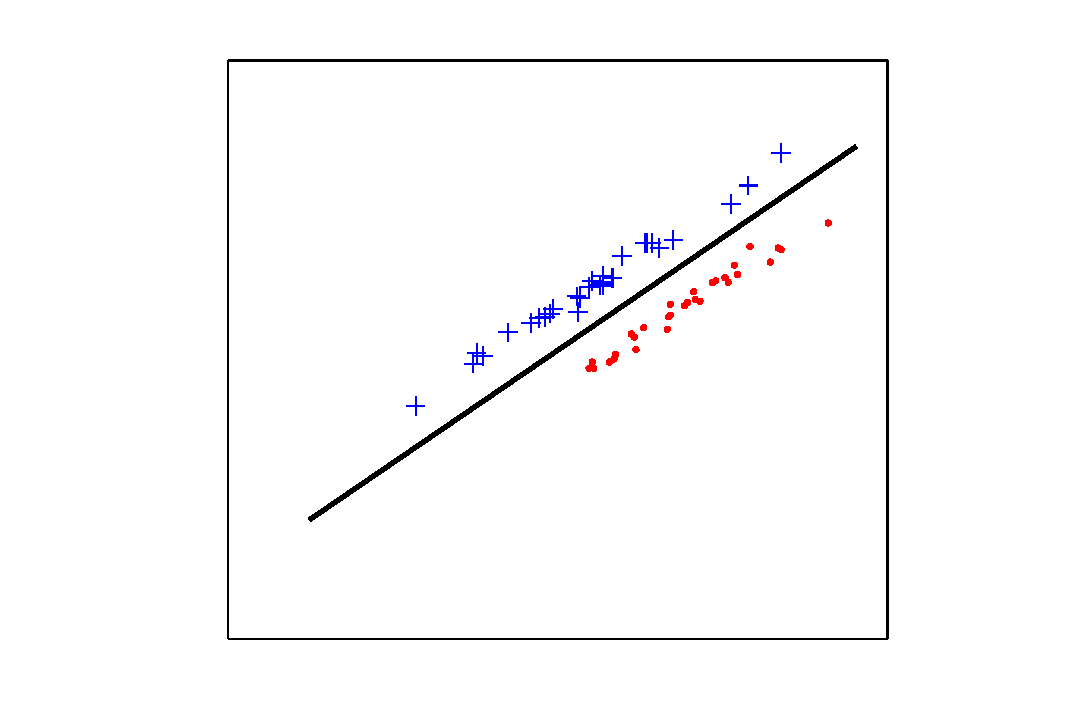
\includegraphics[width=\textwidth]{figures/LDA_boundary.pdf}}
\only<2->{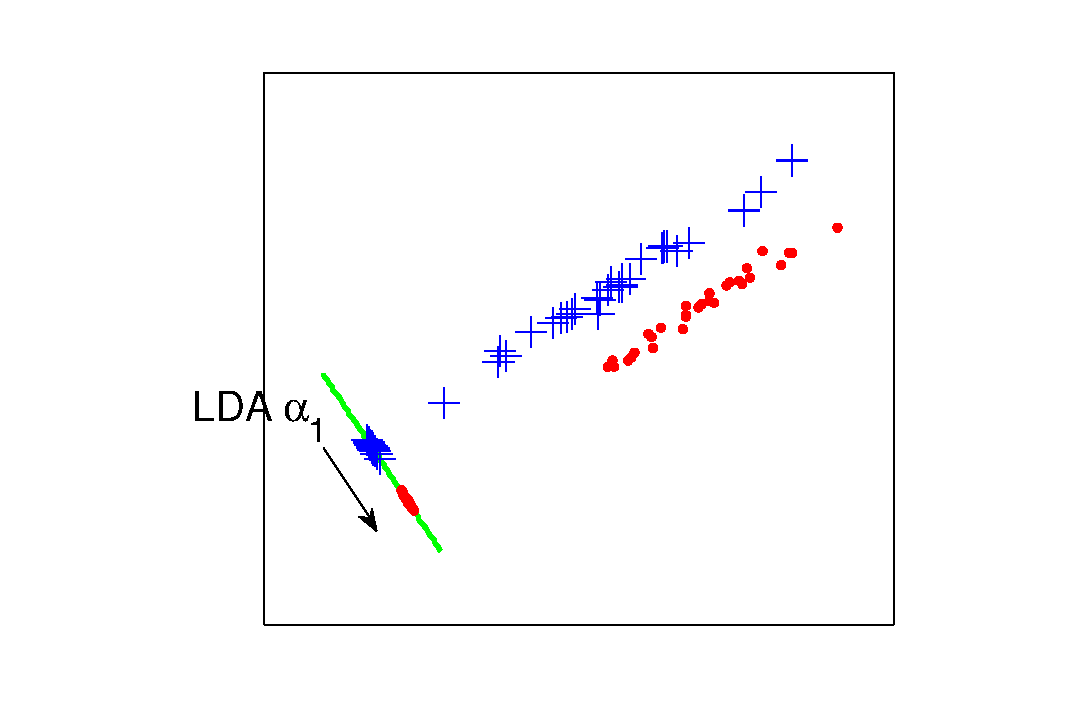
\includegraphics[width=\textwidth]{figures/LDAprojection.pdf} }
\end{column}
\begin{column}{.6\linewidth}
\begin{itemize}
\item LDA: linear decision boundary $a = \vec{w}^\intercal \vLeakVec + w_0$
\pause
\item Equivalently, project data onto $\vec{w}^\intercal \vLeakVec$ (orthogonally to the decision boudary), than classify by a real threshold (optimally $w_0$). \\
\end{itemize}
\end{column}
\end{columns}
\pause
\begin{itemize}
\item Two assumptions about class-conditional densities: 
\begin{itemize}
\item Gaussian distributions with parameters $\mu_j, \Sigma_j$
\item Homoscedasticity: $\Sigma_j=\Sigma$ for all $j$
\end{itemize}
\end{itemize}

\begin{block}{Fact, abuse and preference for the dimensionality reduction formulation}
\begin{itemize}
\item When LDA assumptions are met, the solution $\AAlpha_1$ of the Fisher's criterion is orthogonal to $\vec{w}$. 
\item assumption not required
\item naturally multi-class
\end{itemize}
\end{block}

\end{frame}

\begin{frame}
\frametitle{Linear separability}

\only<1>{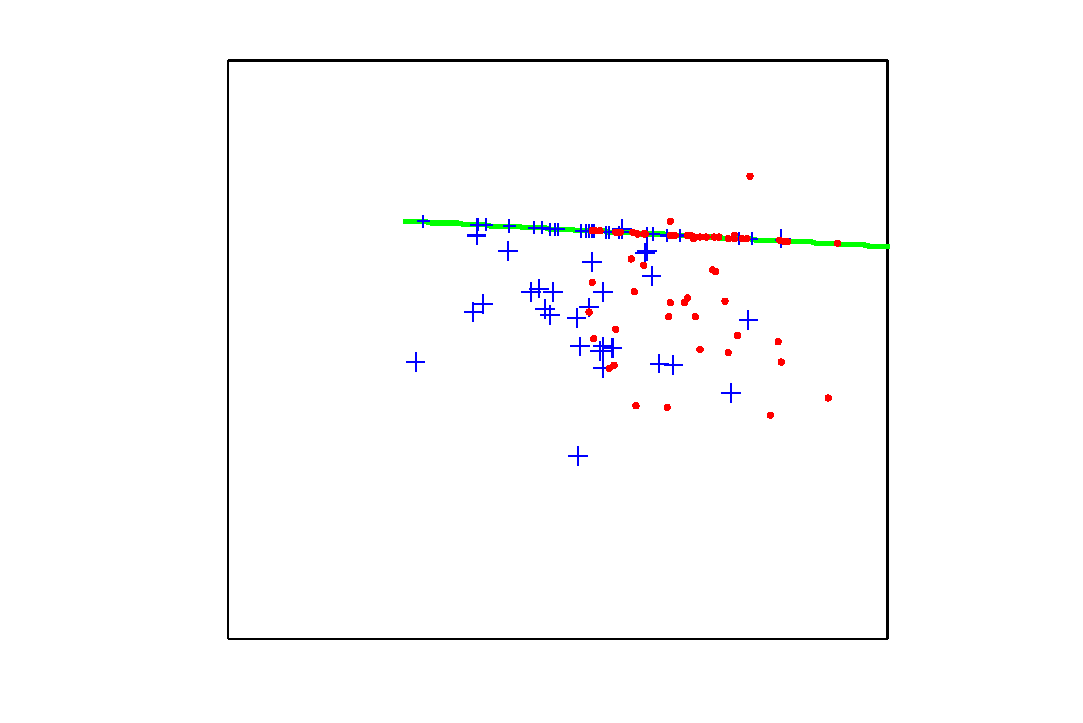
\includegraphics[width=0.5\textwidth]{figures/LDA_non_linearly.pdf}\\ }
LDA: linear decision boundary $a = \vec{w}^\intercal \vLeakVec + w_0$ ($\vec{w} = \Sigma^{-1}(\mu_1-\mu_2)$)
%
\begin{block}{}
\begin{huge}
\centering What if $\mu_1 = \mu_2$? 
\end{huge}
\end{block}
\end{frame}


\begin{frame}
\frametitle{Convolutional Neural Networks}
\vspace*{-10pt}
\begin{block}{Translation-invariance}
\begin{figure}
\centering
\only<1>{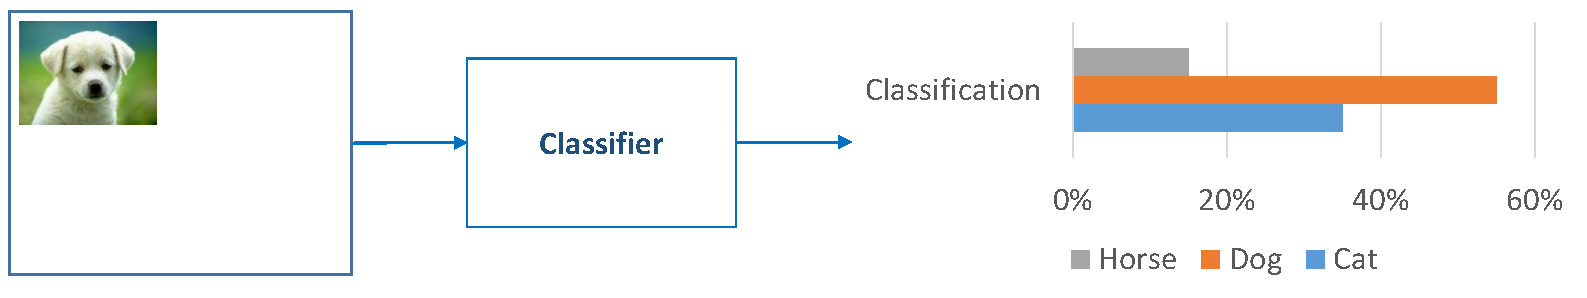
\includegraphics[width=\textwidth]{Figures/cane_shift_classifier1.pdf}}
\only<2>{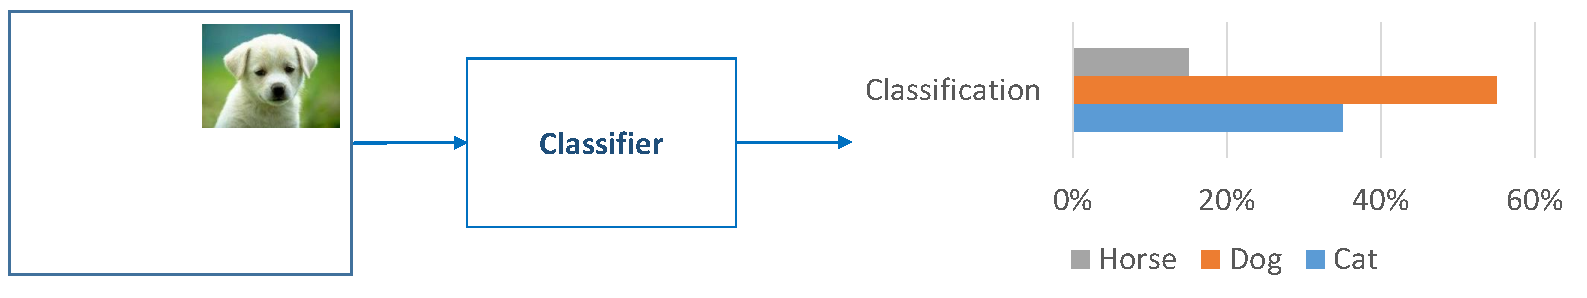
\includegraphics[width=\textwidth]{Figures/cane_shift_classifier2.pdf}}
\only<3-4>{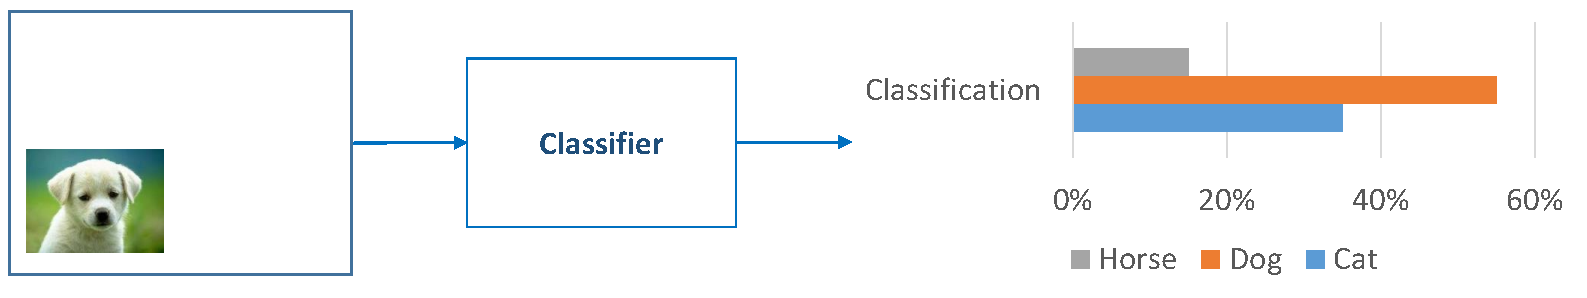
\includegraphics[width=\textwidth]{Figures/cane_shift_classifier3.pdf}}
%\only<5>{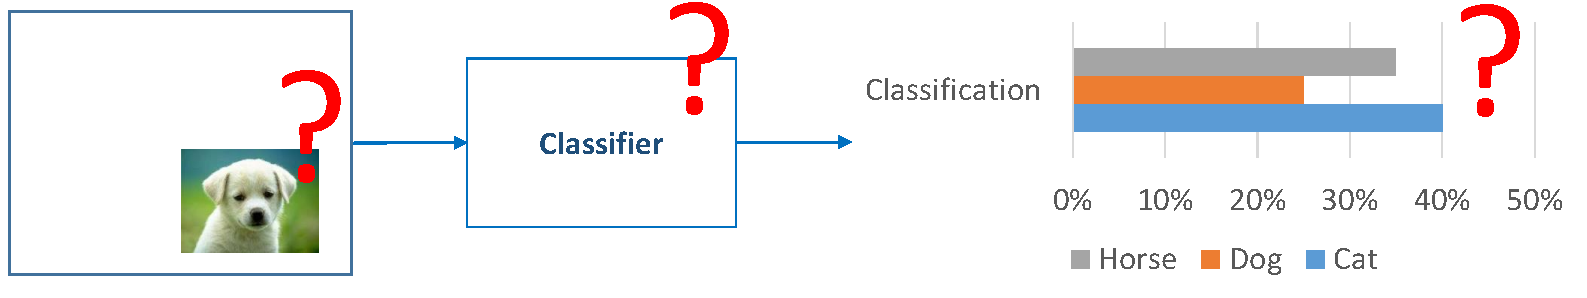
\includegraphics[width=\textwidth]{Figures/cane_shift_classifier4.pdf}}
\only<5>{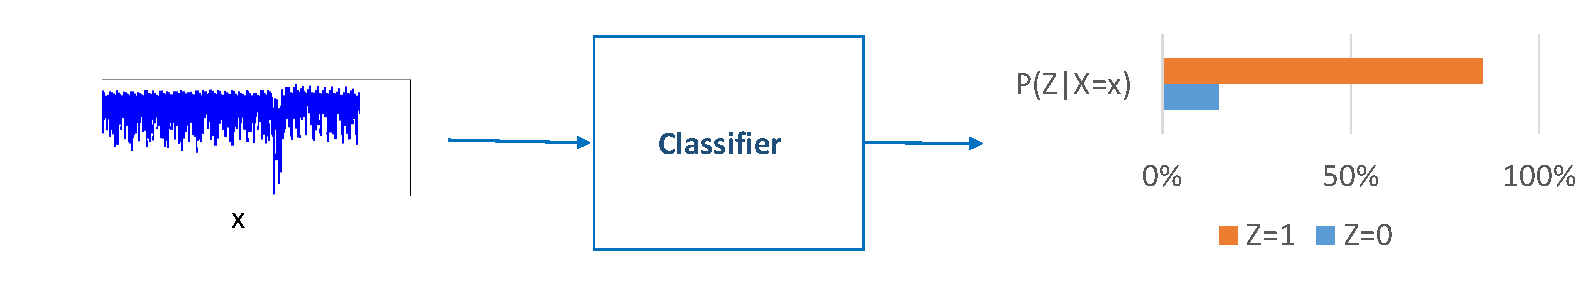
\includegraphics[width=\textwidth]{Figures/trace_shift_classifier1.pdf}}
\only<6>{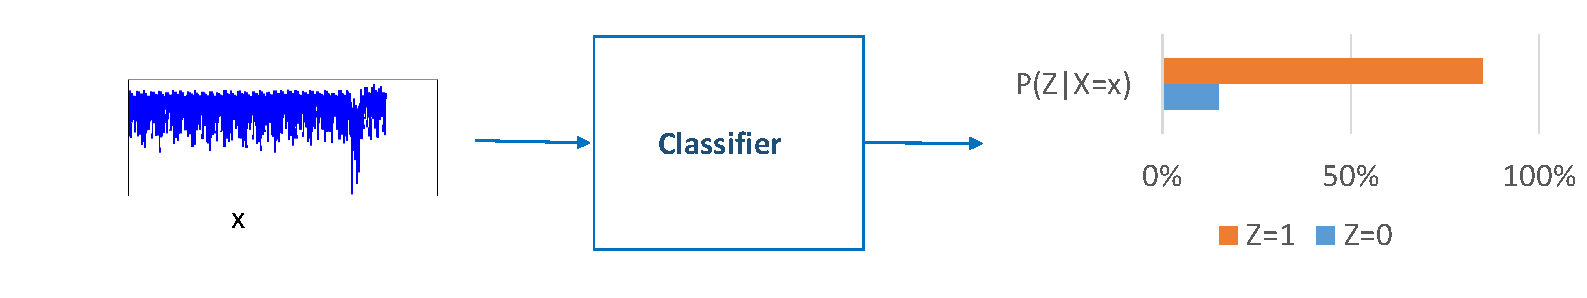
\includegraphics[width=\textwidth]{Figures/trace_shift_classifier2.pdf}}
\only<7->{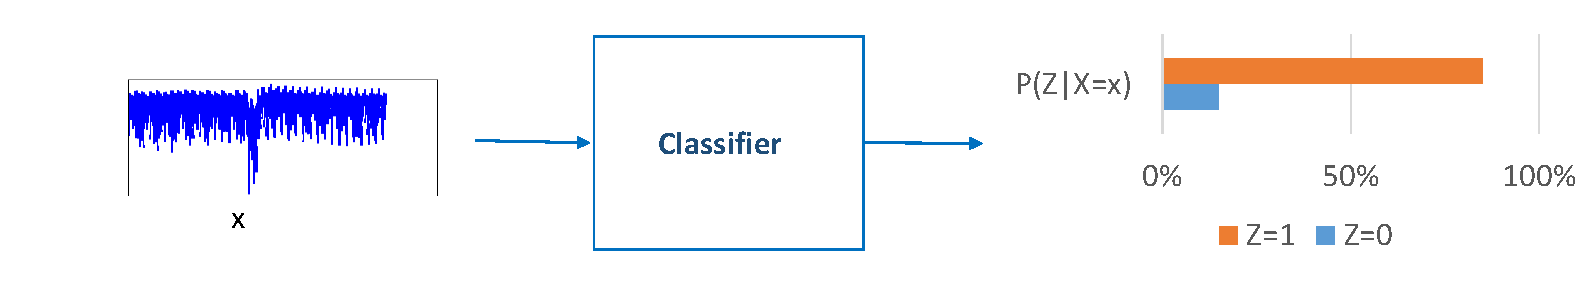
\includegraphics[width=\textwidth]{Figures/trace_shift_classifier3.pdf}}
\end{figure}
\uncover<4->{It is important to explicit the data translation-invariance\\}
\uncover<9->{Convolutional Neural Networks: share weights across space}
\end{block}
%

\vspace*{-7pt}

\begin{columns}
\begin{column}{.5\textwidth}
\only<1-10>{
\begin{figure}

\includegraphics[width=.7\textwidth]{Figures/small_white.pdf}
\end{figure}
}

\only<11>{
\begin{figure}
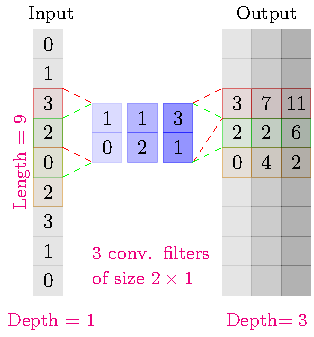
\includegraphics[width=.5\textwidth]{../tikz_per_manuscritto/conv_filter_2_1.pdf} 
\caption{\scriptsize{Linear layer in a ConvNet (\emph{Convolutional Layer})}}
\end{figure}
}

\only<12-13>{
\begin{figure}
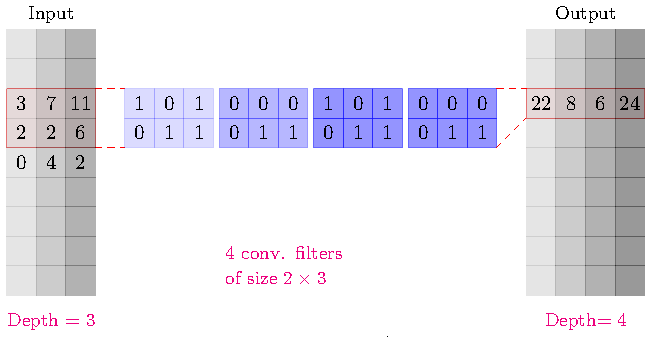
\includegraphics[width=0.8\textwidth]{../tikz_per_manuscritto/conv_filter_2_3.pdf} 
\caption{\scriptsize{Linear layer in a ConvNet (\emph{Convolutional Layer})}}
\end{figure}
}

\end{column}
%%
\begin{column}{.5\textwidth}
\only<1-9>{
\begin{figure}

\includegraphics[width=.7\textwidth]{Figures/big_white.pdf}
\end{figure}}
\only<10-12>{
\begin{figure}
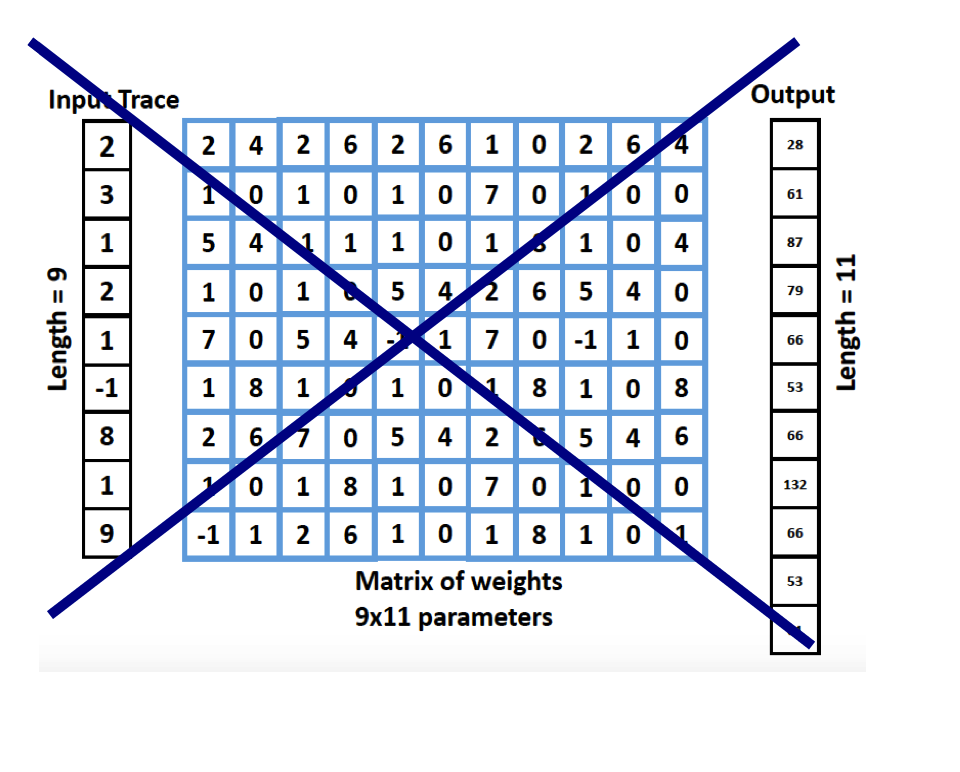
\includegraphics[width=.7\textwidth]{Figures/FC_no.png} 
\caption{\scriptsize{Linear layer in an MLP (\emph{Fully Connected Layer})}}
\end{figure}
}
\only<13->{
\begin{figure}
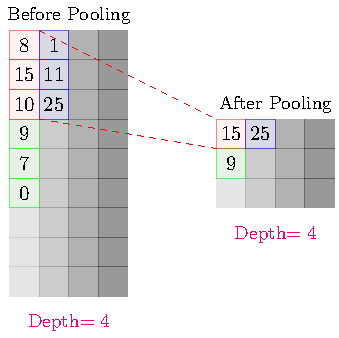
\includegraphics[width=.5\textwidth]{../tikz_per_manuscritto/pooling.pdf} 
\caption{\scriptsize{Max Pooling Layer}}
\end{figure}
}

\end{column}
\end{columns}
\end{frame}

\begin{frame}
\frametitle{Cost function - Cross-entropy}
\vspace*{-3pt}
\begin{itemize}
\item batch of training data $(\vLeakVec_i, \sensVar_i)_{i\in I}$, outputs of the current model $(\vNNOutput_i)_{i\in I}$
\item labels $\sensVar_i=\sensVarValue{j}$ are \emph{one-hot encoded}: $\vec{\sensVar_i} = \sensVarOneHot{j} = (0,\ldots , 0,\underbrace{1}_{j},0,\dots,0)$
\end{itemize}

\begin{block}{Loss function}
\begin{equation}\label{eq:lossfunction}
\mathcal{L} = -\frac{1}{\lvert I \rvert} \sum_{i\in I} \sum_{t=1}^{|\sensVarSet|}\vec{\sensVar_i}[t]\log{\vNNOutput_i[t]}
\end{equation}   
\end{block}

\begin{block}{Maximum-\emph{a-posteriori} or Cross-entropy}
\begin{itemize}
\item $\vNNOutput_i \approx \prob[\given{\sensRandVar}{\vaLeakVec=\vLeakVec_i}]$
\uncover<2>{\item $\vec{\sensVar_i} \approx \prob[\given{\sensRandVar}{\sensRandVar=\sensVarOneHot{j}}]$}
\uncover<2>{\item $\entropy(\vec{\sensVar_i}, \vNNOutput_i) = \entropy(\vec{\sensVar_i}) + D_{KL}(\vec{\sensVar_i} || \vNNOutput_i) = \esper_{\vec{\sensVar_i}}[-\log{\vNNOutput_i}] = -\sum_{t=1}^{|\sensVarSet|}\vec{\sensVar_i}[t]\log{\vNNOutput_i[t]}$}
\only<1>{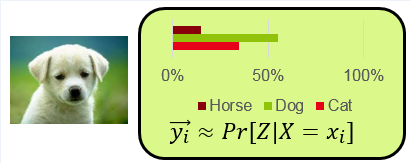
\includegraphics[width=0.4\textwidth]{figures/maxaposteriori.png}}
\only<2>{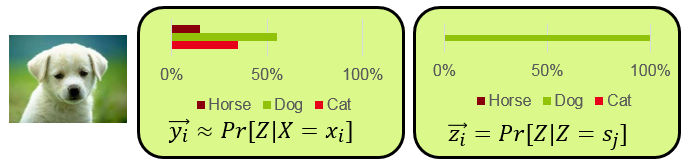
\includegraphics[width=0.7\textwidth]{figures/crossentropy.png}}
\end{itemize}
\end{block}
\end{frame}

\begin{frame}
\frametitle{Capacity-Overfitting-Regularization}


\begin{block}{Regression example}
Performance metric: Mean Square Error (MSE)
\begin{columns}
\begin{column}{.5\textwidth}
\only<1-2>{\begin{figure}
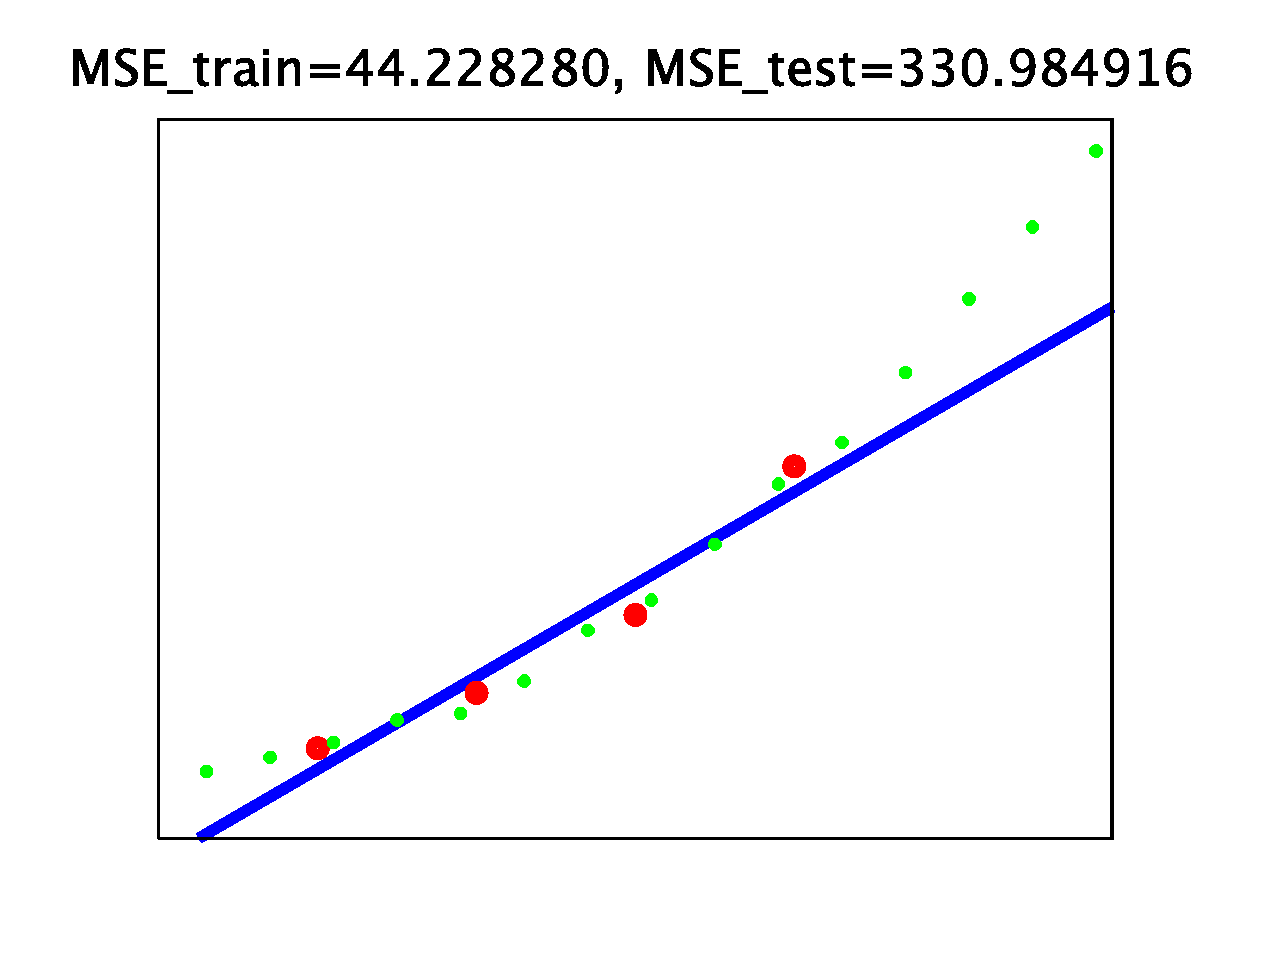
\includegraphics[width=\textwidth]{../Figures/linear_regression.pdf}
\caption{Linear regression $\rightarrow$ underfitting}
\end{figure}}
\only<3-4>{\begin{figure}
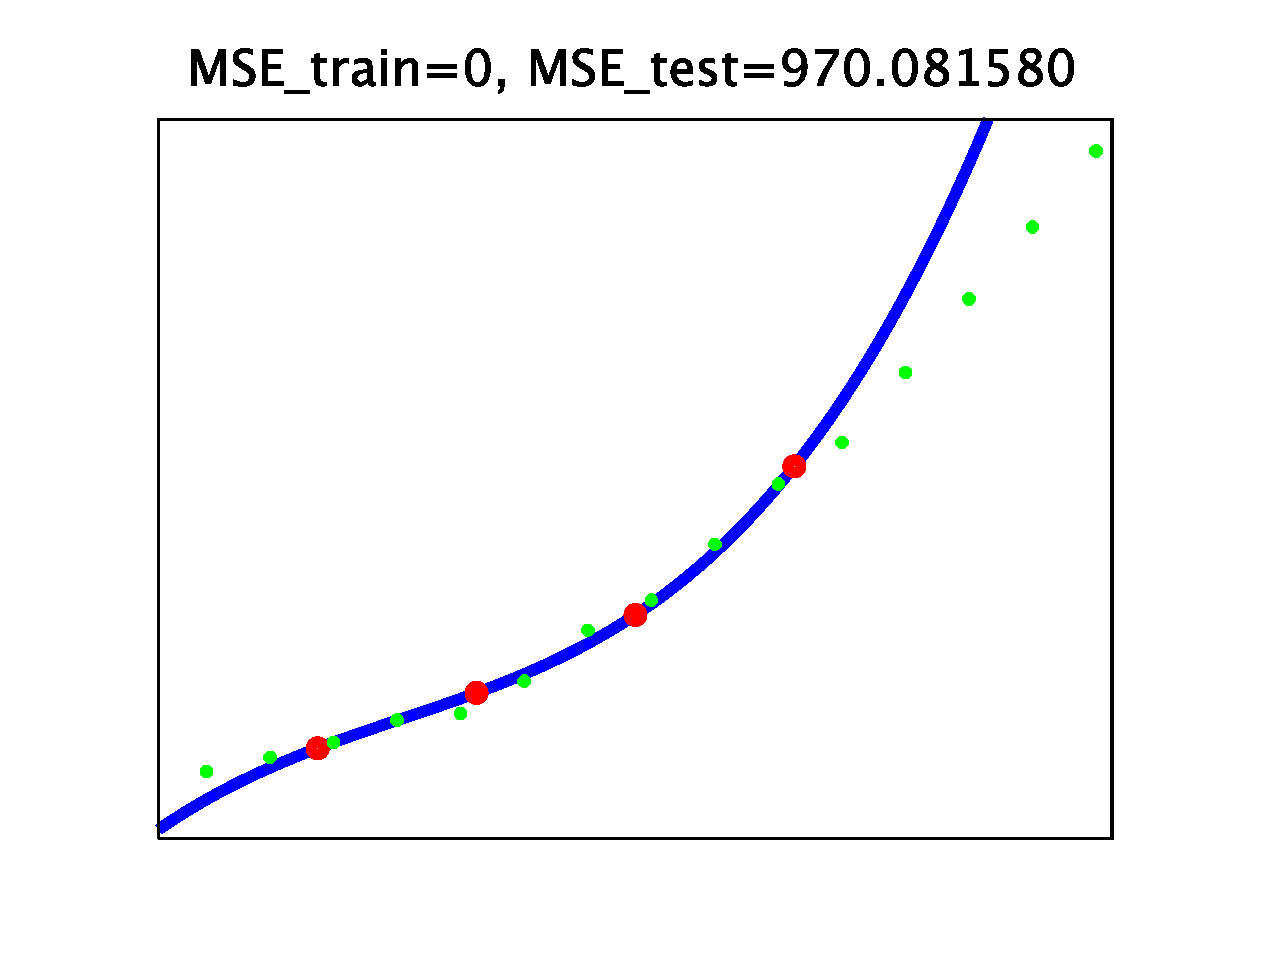
\includegraphics[width=\textwidth]{../Figures/cubic_regression.pdf}
\caption{Cubic regression $\rightarrow$ overfitting}
\end{figure}}
\end{column}
\begin{column}{.5\textwidth}
\only<2-3>{
\begin{figure}
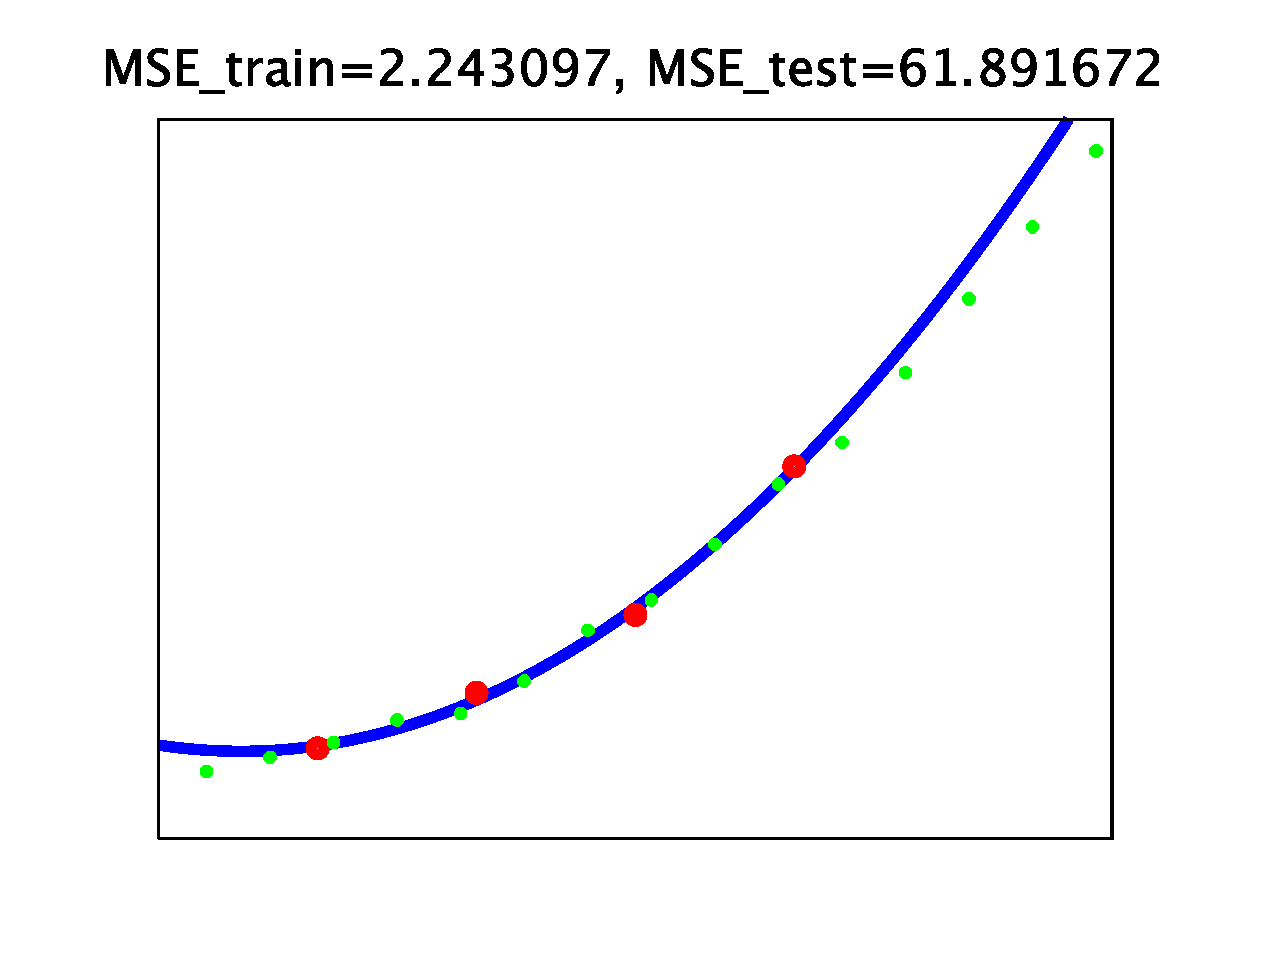
\includegraphics[width=\textwidth]{../Figures/quadratic_regression.pdf}
\caption{Quadratic regression $\rightarrow$ fits}
\end{figure}}
\only<4>{
\begin{figure}
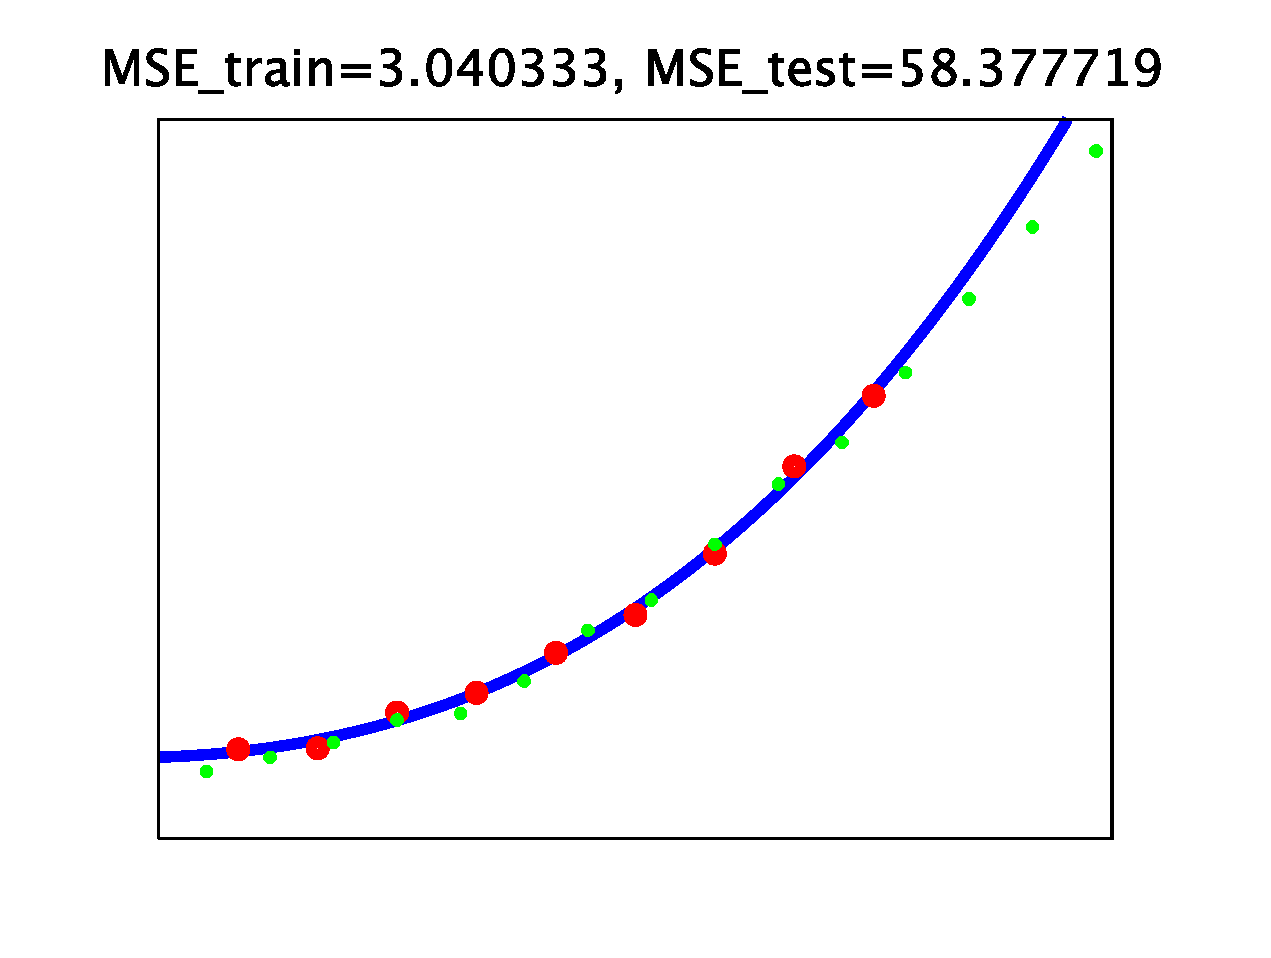
\includegraphics[width=\textwidth]{../Figures/cubic_regression_more.pdf}
\caption{Cubic regression with more training data}
\end{figure}}
\end{column}
\end{columns}
\end{block}

\uncover<5->{
\begin{block}{Classification via Neural Network}
Performance measure: Accuracy (Classification rate)\\
Evaluate and compare training and validation accuracy
\begin{columns}
\begin{column}{.45\textwidth}
\only<5>{Understand significant features
\begin{figure}
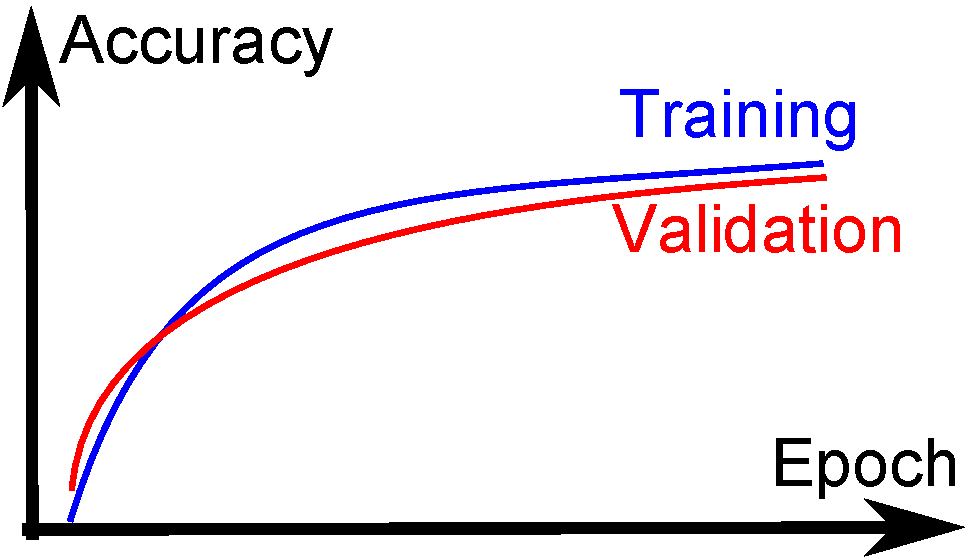
\includegraphics[width=.9\textwidth]{figures/fitting.pdf} 
\end{figure}
}
\only<6>{
Why?
\begin{itemize}
\item[] Too complex model
\item[] Not enough training data
\end{itemize}
Solution? 
\begin{itemize}
\item[] Data augmentation
\end{itemize}
}
\end{column}
\begin{column}{.45\textwidth}
Learn by heart (\textbf{\textcolor{red}{OVERFITTING}})
\begin{figure}
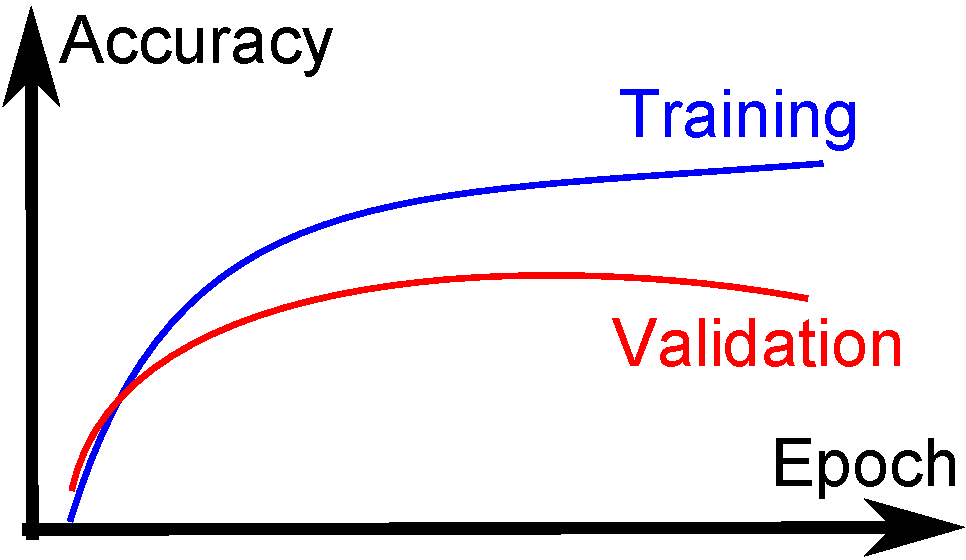
\includegraphics[width=.9\textwidth]{figures/overfitting.pdf} 
\end{figure}

\end{column}
\end{columns}
\end{block}

}



\end{frame}


\begin{frame}
\frametitle{Random Delays - Two Leaking Operations}

\centering
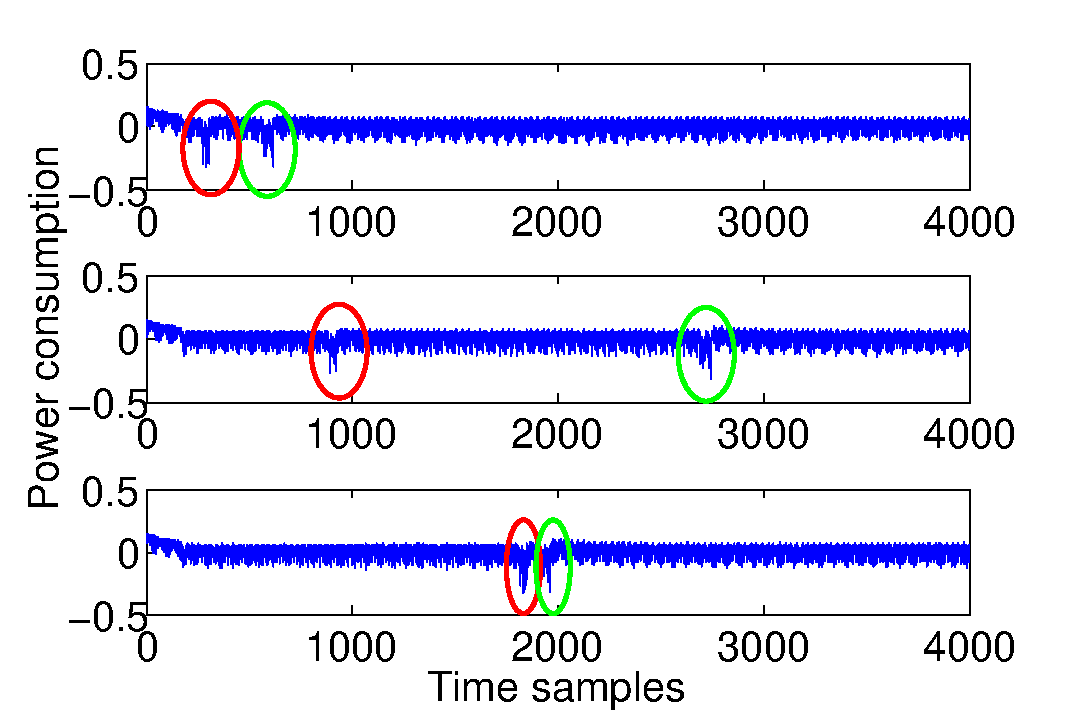
\includegraphics[width=.5\textwidth]{../Figures/CHES2017/CW_double_shift_traces.pdf}	


\begin{block}{Two leaking operations}
First operation - Test acc: $76.8\%$, $N^\star=7$\\
Second operation - Test acc: $82.5\%$, $N^\star=6$
\end{block}

\end{frame}

\begin{frame}
\frametitle{Artificial Jitter}
\begin{figure}
\subfloat[Low artificial jitter]{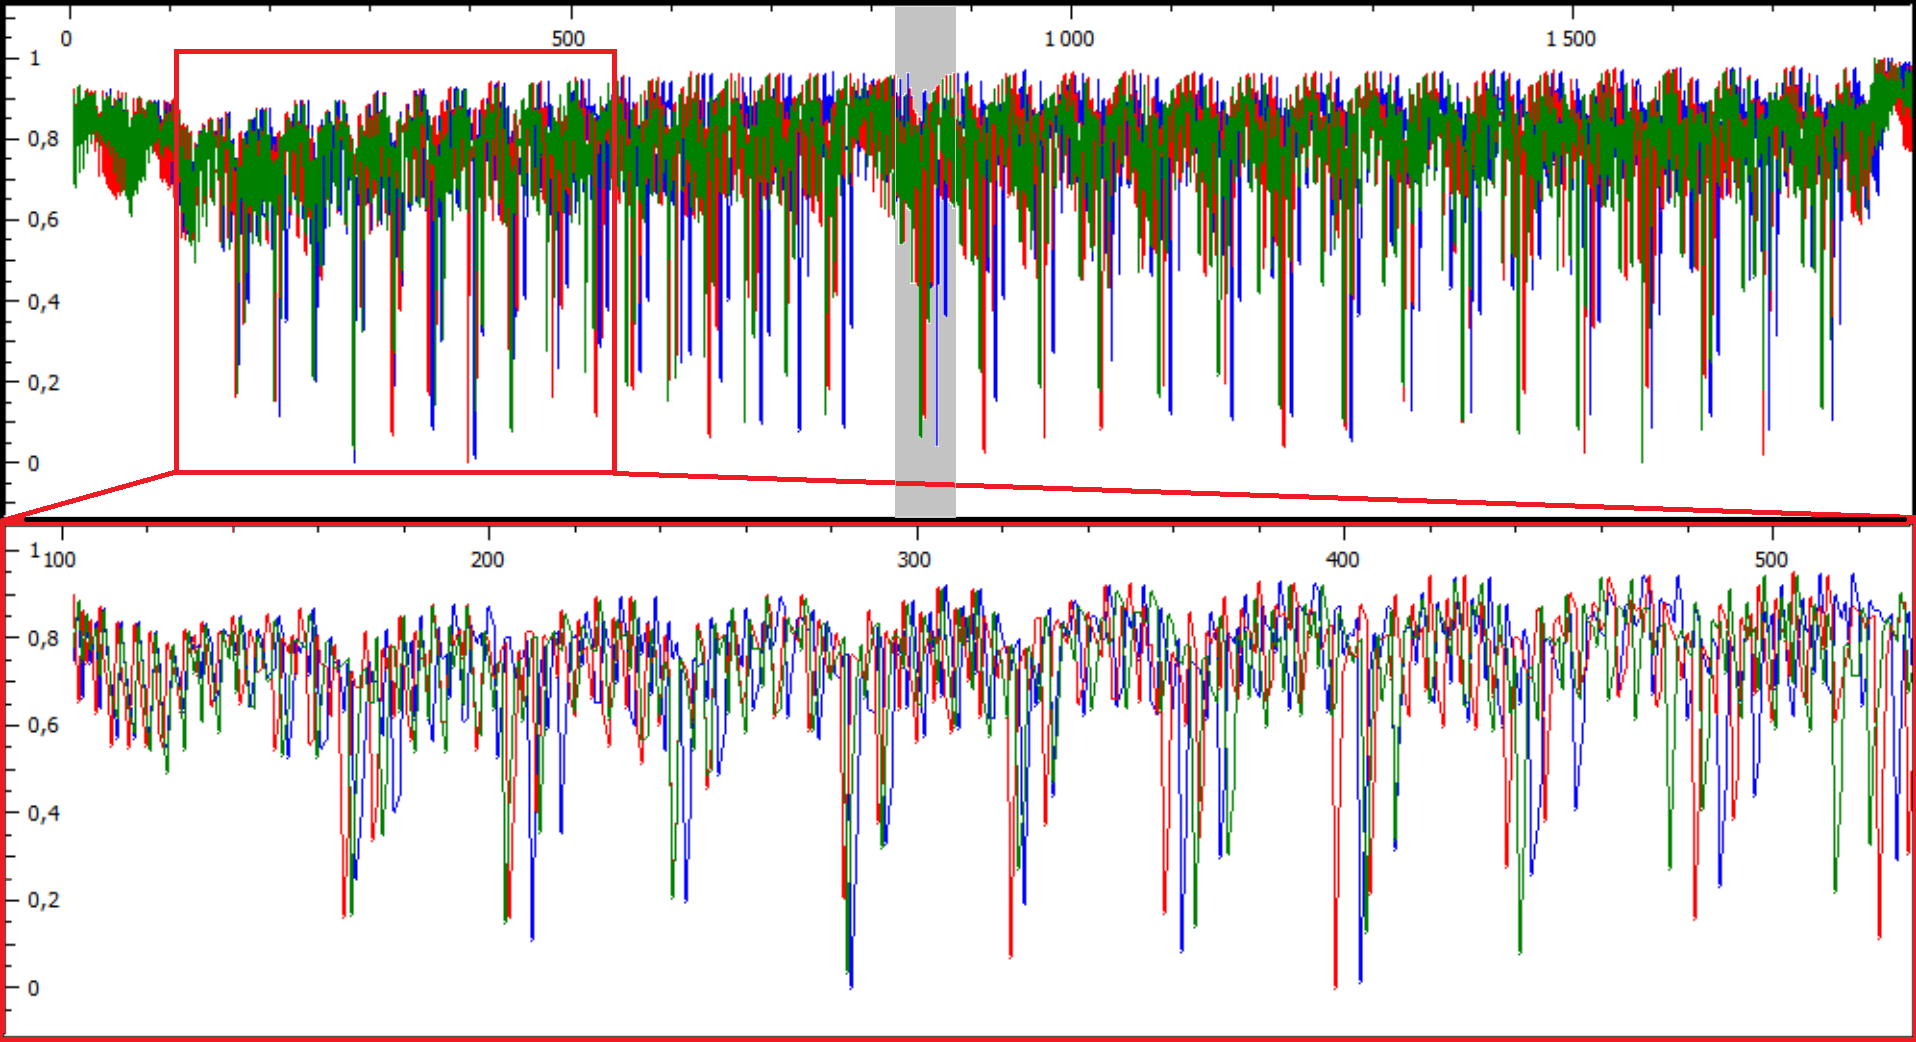
\includegraphics[width=.4\textwidth]{../Figures/CHES2017/jitter_2_2_framed.png} }
\subfloat[High artificial jitter]{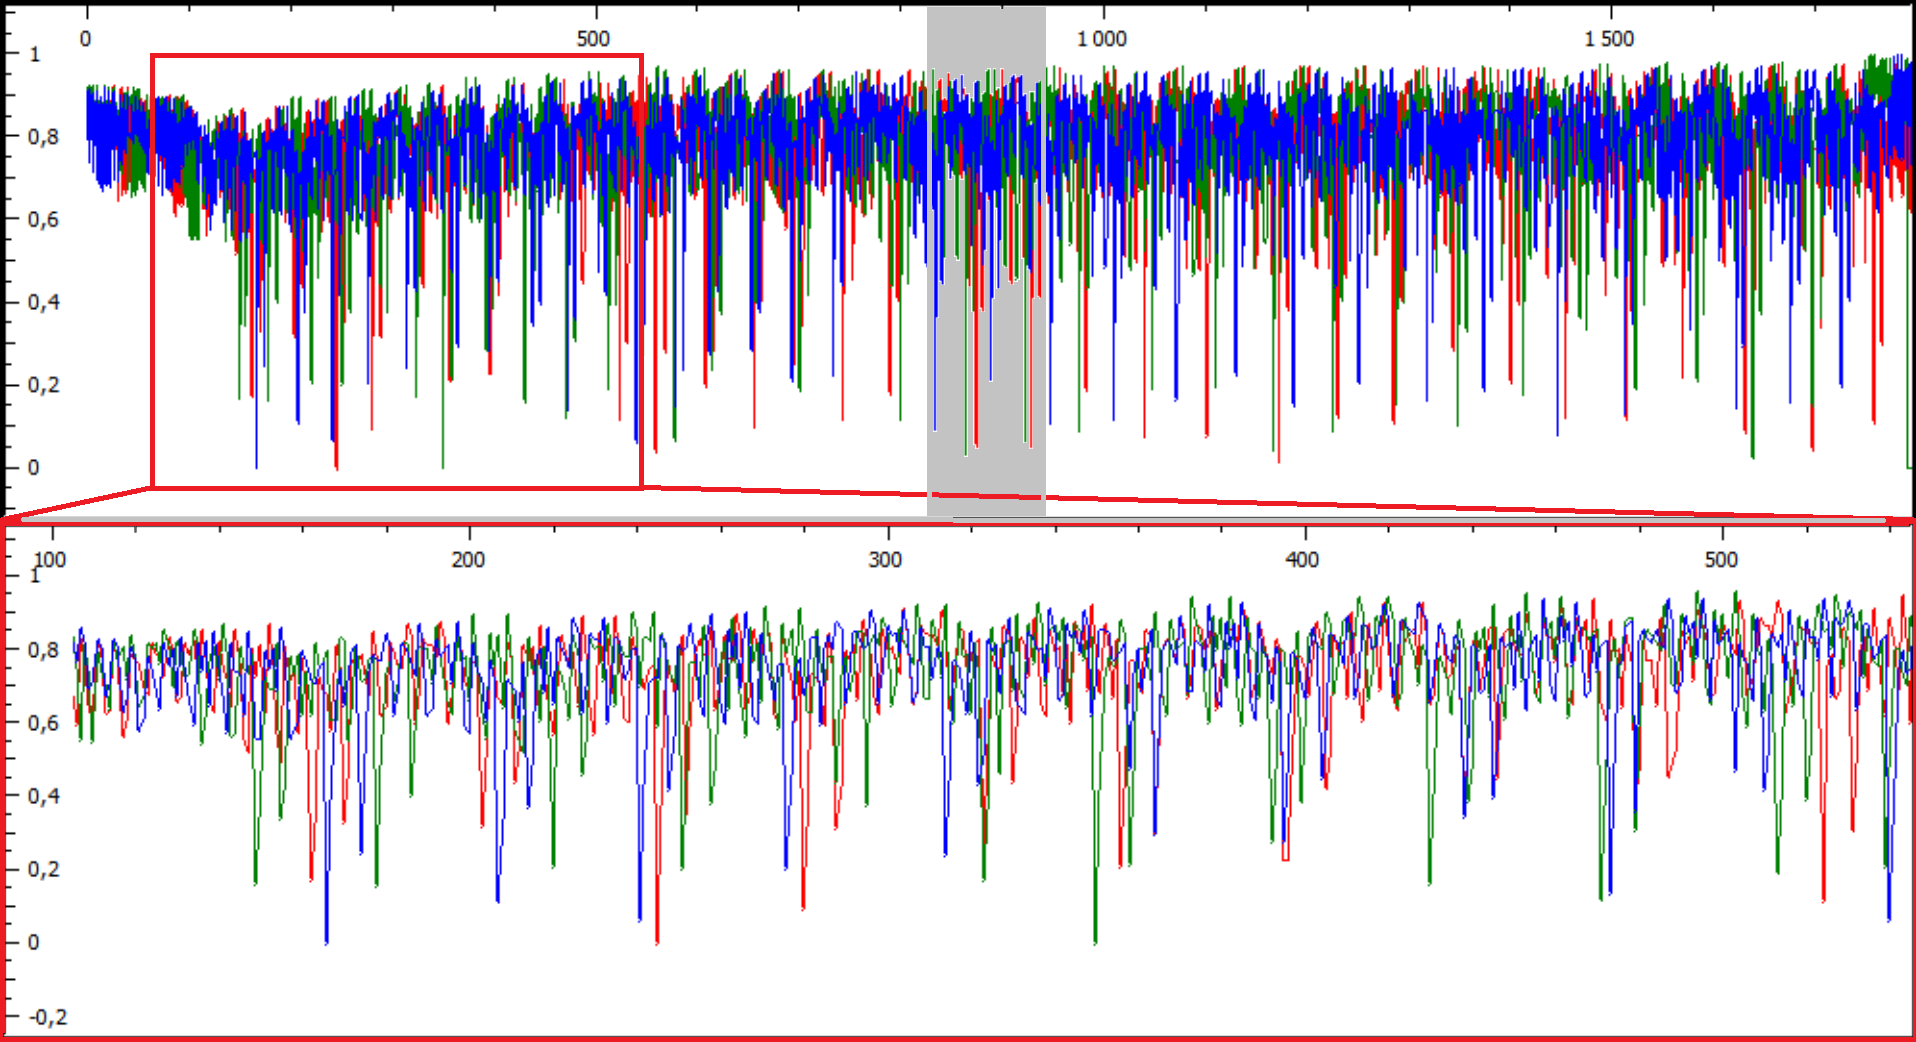
\includegraphics[width=.4\textwidth]{../Figures/CHES2017/jitter_6_6_framed.png} }
\end{figure}
\begin{block}{Target}

\begin{itemize}
\item Target Variable: $Z = \mathrm{HW}(\mathrm{Sbox}(P\oplus K))$
\item $\approx 2000$ time samples
\item Countermeasure: artificial signal treatment simulating clock jitter
\item 10000 training traces
\end{itemize}
\end{block}


\end{frame}

\begin{frame}
\frametitle{Artificial Jitter (2)}
\vspace*{-10pt}
\begin{scriptsize}
\newcolumntype{C}{>{\centering\arraybackslash}p{3em}}
\begin{table}[t]
\centering

\begin{tabular}{|C|C|CCCCCC|}
\multicolumn{8}{C}{\emph{Low\_jitter}}      \\                                            
\hline
Acc                          & $N^\star$                         & \multicolumn{2}{C|}{$\mathrm{SH}_{0}$}                                                   & \multicolumn{2}{C|}{$\mathrm{SH}_{20}$}                                                & \multicolumn{2}{C|}{$\mathrm{SH}_{40}$}                                           \\ \hline
\multicolumn{2}{|C|}{$\mathrm{AR}_{0}$}   & \multicolumn{1}{C|}{\cellcolor[HTML]{EFEFEF}57.4\%}  & \multicolumn{1}{C|}{\cellcolor[HTML]{EFEFEF}14}     & \multicolumn{1}{C|}{82.5\%}                         & \multicolumn{1}{C|}{6}                              & \multicolumn{1}{C|}{83.6\%}                                  & 6                                                            \\ \cline{1-8}
\multicolumn{2}{|C|}{$\mathrm{AR}_{100}$} & \multicolumn{1}{C|}{86.0\%}                          & \multicolumn{1}{C|}{6}                              & \multicolumn{1}{C|}{87.0\%}                         & \multicolumn{1}{C|}{5}                              & \multicolumn{1}{C|}{87.5\%}                                  & 6                                                             \\ \cline{1-8}
\multicolumn{2}{|C|}{$\mathrm{AR}_{200}$} & \multicolumn{1}{C|}{86.6\%}                          & \multicolumn{1}{C|}{6}                              & \multicolumn{1}{C|}{85.7\%} & \multicolumn{1}{C|}{6}      & \multicolumn{1}{C|}{\textbf{87.7\%}} & \textbf{5}      \\ \hline


\end{tabular}


\end{table}
\begin{table}[t]
\centering


\begin{tabular}{|C|C|CCCCCC|}
\multicolumn{8}{C}{\emph{High\_jitter}}      \\   
\hline
Acc                          & $N^\star$                         & \multicolumn{2}{C|}{$\mathrm{SH}_{0}$}                                                   & \multicolumn{2}{C|}{$\mathrm{SH}_{20}$}                                              & \multicolumn{2}{C|}{$\mathrm{SH}_{40}$}                                             \\ \hline
\multicolumn{2}{|C|}{$\mathrm{AR}_{0}$}   & \multicolumn{1}{C|}{\cellcolor[HTML]{EFEFEF}40.6\%} & \multicolumn{1}{C|}{\cellcolor[HTML]{EFEFEF}35}  & \multicolumn{1}{C|}{51.1\%} & \multicolumn{1}{C|}{9}      & \multicolumn{1}{C|}{62.4\%}           & 11                                 \\ \cline{1-8}
\multicolumn{2}{|C|}{$\mathrm{AR}_{100}$} & \multicolumn{1}{C|}{50.2\%} & \multicolumn{1}{C|}{15}     & \multicolumn{1}{C|}{72.4\%} & \multicolumn{1}{C|}{11}     & \multicolumn{1}{C|}{73.5\%}           & 9                       \\ \cline{1-8}
\multicolumn{2}{|C|}{$\mathrm{AR}_{200}$} & \multicolumn{1}{C|}{64.0\%} & \multicolumn{1}{C|}{11}     & \multicolumn{1}{C|}{\textbf{75.5\%}} & \multicolumn{1}{C|}{\textbf{8}}   & \multicolumn{1}{C|}{74.4\%}           & 8           \\ \hline


\end{tabular}


\end{table}
\end{scriptsize}


\begin{figure}
\subfloat[Low Jitter]{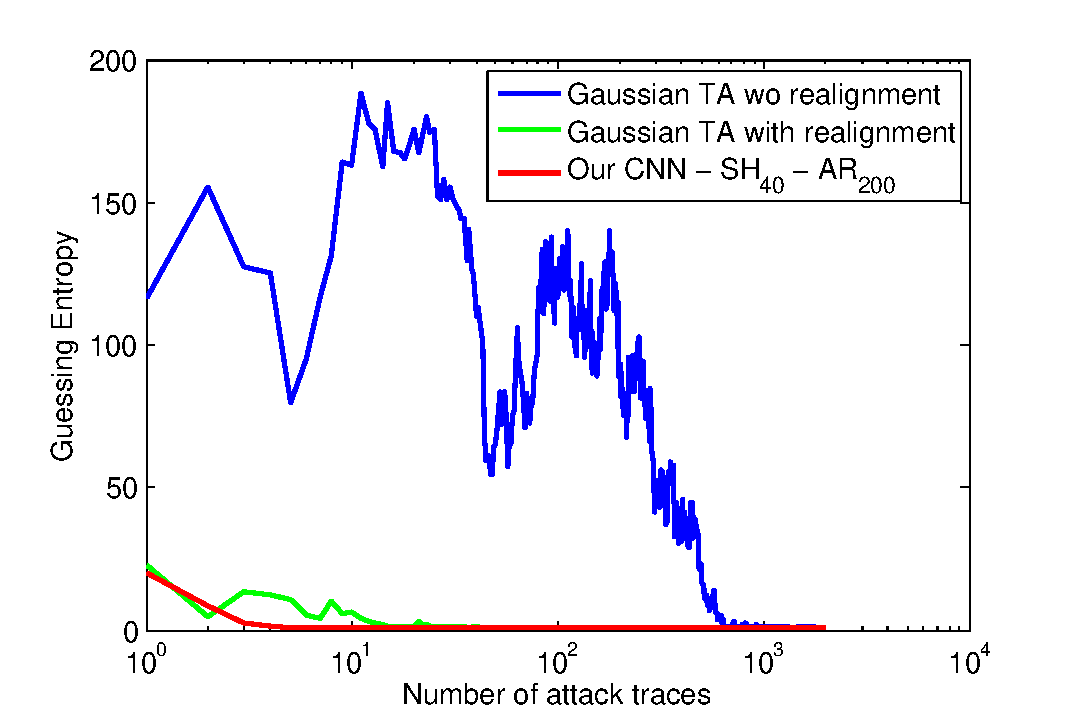
\includegraphics[width=.45\textwidth]{../Figures/CHES2017/results_low_jitter_new.pdf} }
\subfloat[High Jitter]{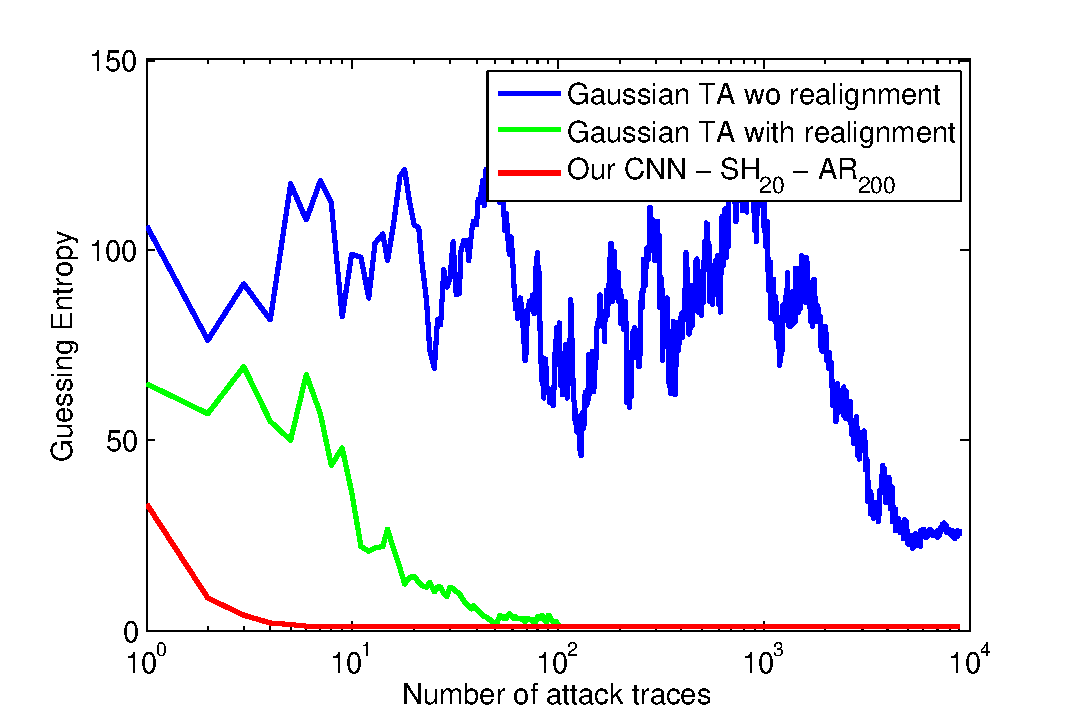
\includegraphics[width=.45\textwidth]{../Figures/CHES2017/results_high_jitter_new.pdf} }

\end{figure}
\end{frame}



\begin{frame}
\frametitle{Artificial Jitter}
\begin{tiny}

\newcolumntype{C}{>{\centering\arraybackslash}p{3em}}
\begin{table}[t]
\centering
\label{table:results_all}



\begin{tabular}{|C|C|CCCCCC|CC}
\hline
\multicolumn{10}{|C|}{\textbf{\emph{DS\_low\_jitter}}}\\
\hline
$a$                           & $b$                         & \multicolumn{2}{C|}{}                                                                                      & \multicolumn{2}{C|}{}                                                                                     & \multicolumn{2}{C|}{}                                                                                  & \multicolumn{2}{C|}{}                                      \\ \cline{1-2}
$c$                           & $d$                         & \multicolumn{2}{C|}{\multirow{-2}{*}{$\mathrm{SH}_{0}$}}                                                   & \multicolumn{2}{c|}{\multirow{-2}{*}{$\mathrm{SH}_{20}$}}                                                 & \multicolumn{2}{c|}{\multirow{-2}{*}{$\mathrm{SH}_{40}$}}                                              & \multicolumn{2}{c|}{\multirow{-2}{*}{$\mathrm{SH}_{200}$}} \\ \hline
\multicolumn{2}{|c|}{}                                      & \multicolumn{1}{c|}{\cellcolor[HTML]{EFEFEF}100.0\%} & \multicolumn{1}{c|}{\cellcolor[HTML]{EFEFEF}68.7\%} & \multicolumn{1}{c|}{99.8\%}                         & \multicolumn{1}{c|}{86.1\%}                         & \multicolumn{1}{c|}{98.9\%}                                  & 84.1\%                                  &                              &                             \\ \cline{3-8}
\multicolumn{2}{|c|}{\multirow{-2}{*}{$\mathrm{AR}_{0}$}}   & \multicolumn{1}{c|}{\cellcolor[HTML]{EFEFEF}57.4\%}  & \multicolumn{1}{c|}{\cellcolor[HTML]{EFEFEF}14}     & \multicolumn{1}{c|}{82.5\%}                         & \multicolumn{1}{c|}{6}                              & \multicolumn{1}{c|}{83.6\%}                                  & 6                                       &                              &                             \\ \cline{1-8}
\multicolumn{2}{|c|}{}                                      & \multicolumn{1}{c|}{87.7\%}                          & \multicolumn{1}{c|}{88.2\%}                         & \multicolumn{1}{c|}{82.4\%}                         & \multicolumn{1}{c|}{88.4\%}                         & \multicolumn{1}{c|}{81.9\%}                                  & 89.6\%                                  &                              &                             \\ \cline{3-8}
\multicolumn{2}{|c|}{\multirow{-2}{*}{$\mathrm{AR}_{100}$}} & \multicolumn{1}{c|}{86.0\%}                          & \multicolumn{1}{c|}{6}                              & \multicolumn{1}{c|}{87.0\%}                         & \multicolumn{1}{c|}{5}                              & \multicolumn{1}{c|}{87.5\%}                                  & 6                                       &                              &                             \\ \cline{1-8}
\multicolumn{2}{|c|}{}                                      & \multicolumn{1}{c|}{83.2\%}                          & \multicolumn{1}{c|}{88.6\%}                         & \multicolumn{1}{c|}{81.4\%} & \multicolumn{1}{c|}{86.9\%} & \multicolumn{1}{c|}{\textbf{80.6\%}} &\textbf{88.9\%} &                              &                             \\ \cline{3-8}
\multicolumn{2}{|c|}{\multirow{-2}{*}{$\mathrm{AR}_{200}$}} & \multicolumn{1}{c|}{86.6\%}                          & \multicolumn{1}{c|}{6}                              & \multicolumn{1}{c|}{85.7\%} & \multicolumn{1}{c|}{6}      & \multicolumn{1}{c|}{\textbf{87.7\%}} & \textbf{5}      &                              &                             \\ \hline
\multicolumn{2}{|c|}{}                                      &                                                      &                                                     &                                                     &                                                     &                                                              &                                         & \multicolumn{1}{c|}{85.0\%}  & \multicolumn{1}{c|}{88.6\%} \\ \cline{9-10} 
\multicolumn{2}{|c|}{\multirow{-2}{*}{$\mathrm{AR}_{500}$}} &                                                      &                                                     &                                                     &                                                     &                                                              &                                         & \multicolumn{1}{c|}{86.2\%}  & \multicolumn{1}{c|}{5}      \\ \cline{1-2} \cline{9-10}
\multicolumn{10}{|C|}{}\\
\hline
\multicolumn{10}{|C|}{\textbf{\emph{DS\_high\_jitter}}}\\
\hline
$a$                          & $b$                         & \multicolumn{2}{C|}{\multirow{2}{*}{$\mathrm{SH}_{0}$}}   & \multicolumn{2}{C|}{\multirow{2}{*}{$\mathrm{SH}_{20}$}}  & \multicolumn{2}{C|}{\multirow{2}{*}{$\mathrm{SH}_{40}$}} & \multicolumn{2}{C|}{\multirow{2}{*}{$\mathrm{SH}_{200}$}} \\ \cline{1-2}
$c$                          & $d$                         & \multicolumn{2}{C|}{}                                     & \multicolumn{2}{C|}{}                                     & \multicolumn{2}{C|}{}                                    & \multicolumn{2}{C|}{}                                     \\ \hline
\multicolumn{2}{|C|}{\multirow{2}{*}{$\mathrm{AR}_{0}$}}   & \multicolumn{1}{C|}{\cellcolor[HTML]{EFEFEF}100\%}  & \multicolumn{1}{l|}{\cellcolor[HTML]{EFEFEF}45.0\%} & \multicolumn{1}{C|}{100\%}  & \multicolumn{1}{C|}{60.0\%} & \multicolumn{1}{l|}{98.5\%}           & 67.6\%           &                             &                             \\ \cline{3-8}
\multicolumn{2}{|C|}{}                                     &  \multicolumn{1}{C|}{\cellcolor[HTML]{EFEFEF}40.6\%} & \multicolumn{1}{C|}{\cellcolor[HTML]{EFEFEF}35}  & \multicolumn{1}{C|}{51.1\%} & \multicolumn{1}{C|}{9}      & \multicolumn{1}{C|}{62.4\%}           & 11               &                             &                             \\ \cline{1-8}
\multicolumn{2}{|C|}{\multirow{2}{*}{$\mathrm{AR}_{100}$}} & \multicolumn{1}{C|}{90.4\%} & \multicolumn{1}{l|}{57.3\%} & \multicolumn{1}{C|}{76.6\%} & \multicolumn{1}{C|}{73.6\%} & \multicolumn{1}{C|}{78.5\%}           & 76.4\%           &                             &                             \\ \cline{3-8}
\multicolumn{2}{|C|}{}                                     & \multicolumn{1}{C|}{50.2\%} & \multicolumn{1}{C|}{15}     & \multicolumn{1}{C|}{72.4\%} & \multicolumn{1}{C|}{11}     & \multicolumn{1}{C|}{73.5\%}           & 9                &                             &                             \\ \cline{1-8}
\multicolumn{2}{|C|}{\multirow{2}{*}{$\mathrm{AR}_{200}$}} & \multicolumn{1}{C|}{83.1\%} & \multicolumn{1}{C|}{67.7\%} &\multicolumn{1}{C|}{\textbf{82.0\%}} & \multicolumn{1}{C|}{\textbf{77.1\%}} & \multicolumn{1}{l|}{82.6\%}           & 77.0\%           &                             &                             \\ \cline{3-8}
\multicolumn{2}{|C|}{}                                     & \multicolumn{1}{C|}{64.0\%} & \multicolumn{1}{C|}{11}     & \multicolumn{1}{C|}{\textbf{75.5\%}} & \multicolumn{1}{C|}{\textbf{8}}   & \multicolumn{1}{C|}{74.4\%}           & 8                &                             &                             \\ \hline
\multicolumn{2}{|C|}{\multirow{2}{*}{$\mathrm{AR}_{500}$}} &                             &                             &                             &                             &                                       &                  & \multicolumn{1}{C|}{83.6\%} & \multicolumn{1}{C|}{73.4\%} \\ \cline{9-10} 
\multicolumn{2}{|C|}{}                                     &                             &                             &                             &                             &                                       &                  & \multicolumn{1}{C|}{68.2\%} & \multicolumn{1}{C|}{11}     \\ \cline{1-2} \cline{9-10}  
\end{tabular}


\end{table}

\end{tiny}
\end{frame}




\begin{frame}
\frametitle{Real Jitter (1)}
\vspace{-10pt}
\begin{block}{Target}
\begin{itemize}
\item AES hardware implementation
\item strong jitter effect
\item Target Variable: $Z = \mathrm{Sbox}(P\oplus K)$
\item $2,500$ selected time samples
\item $99,000$ training traces
\end{itemize}
\end{block}

\only<1>{
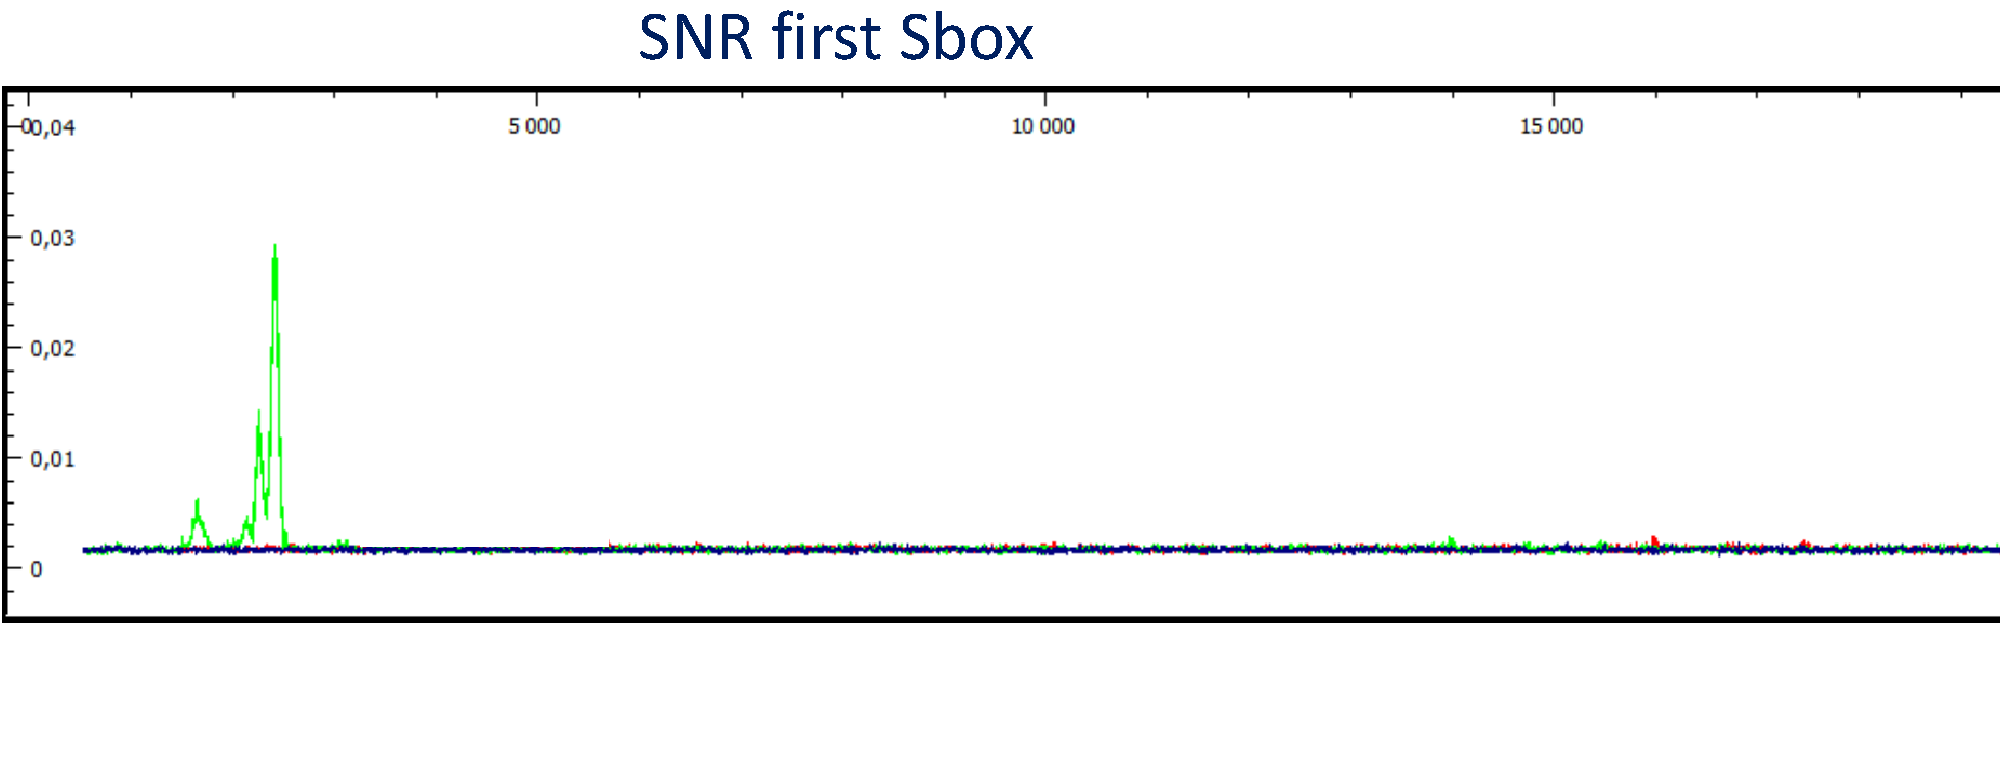
\includegraphics[width=\textwidth]{../Figures/CHES2017/SNR_firstSbox.pdf}
}
\only<2>{
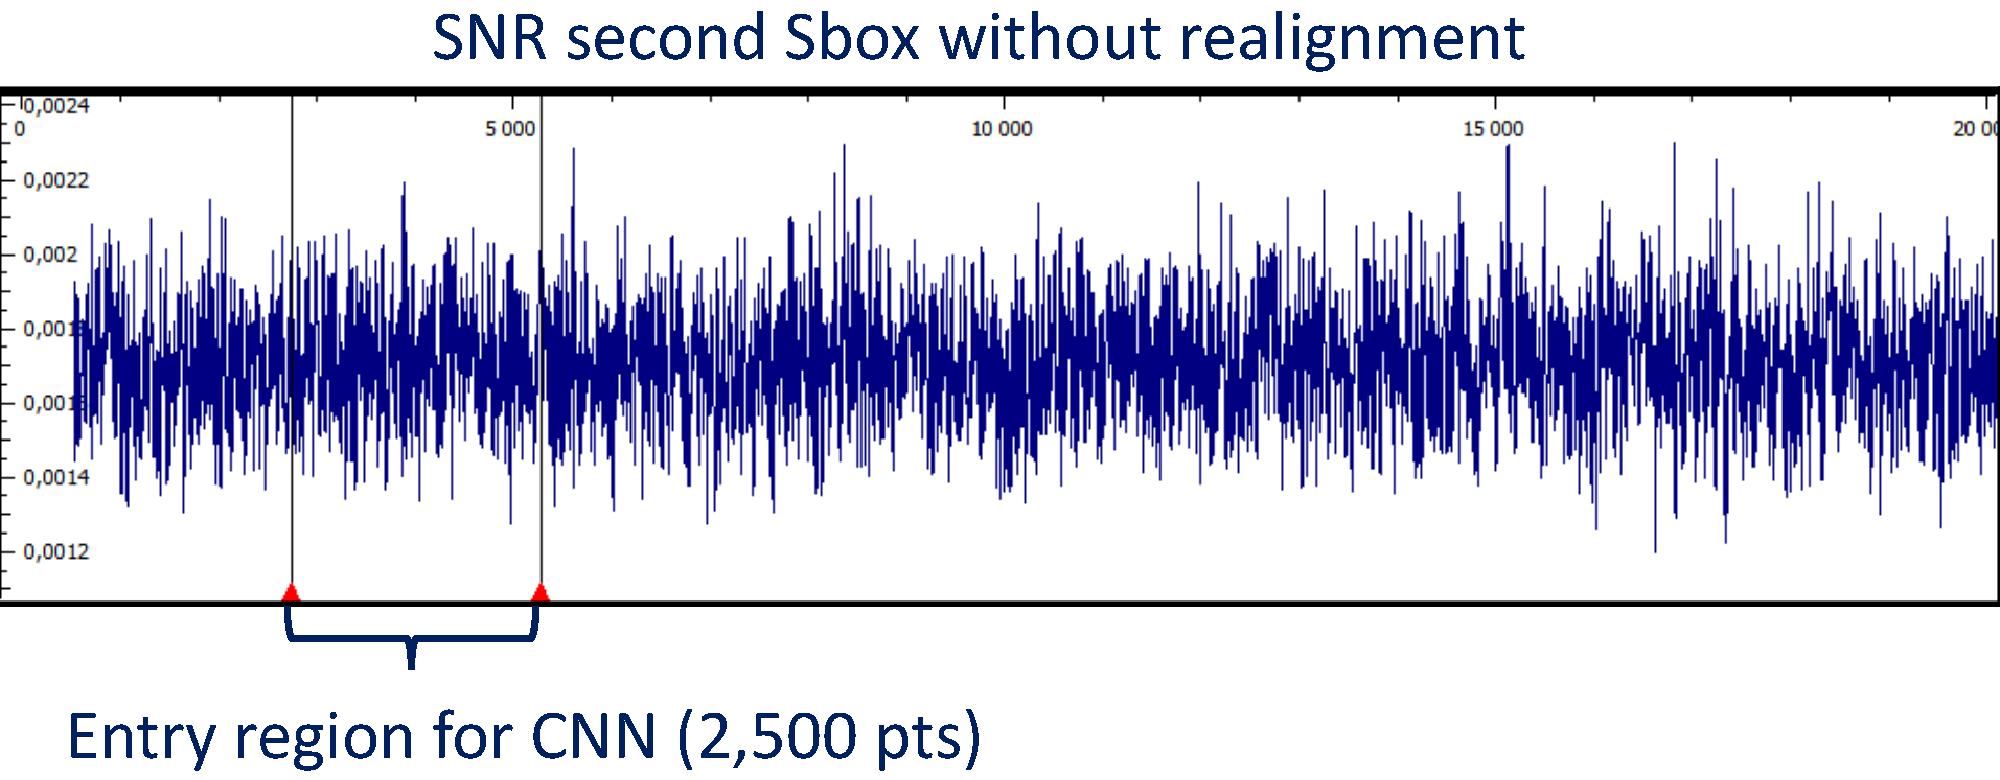
\includegraphics[width=\textwidth]{../Figures/CHES2017/SNR_desynchro.pdf}
}



\end{frame}

\begin{frame}
\frametitle{Real Jitter (2)}
\centering
\begin{scriptsize}
\begin{table}
\begin{tabular}{|c|c|c|c|c|c|c|c|}
\multicolumn{8}{c}{}\\
\hline
\multicolumn{2}{|c|}{} & \multicolumn{2}{c|}{\textcolor{green}{$\mathrm{SH}_{0}$}\textcolor{blue}{$\mathrm{AR}_{0}$}} & \multicolumn{2}{c|}{\textcolor{green}{$\mathrm{SH}_{10}$}\textcolor{blue}{$\mathrm{AR}_{100}$}} & \multicolumn{2}{c|}{\textcolor{green}{$\mathrm{SH}_{20}$}\textcolor{blue}{$\mathrm{AR}_{200}$}} \\ \hline
Acc        & $N^\star$       & 1.2\%                      & 137                      & 1.3\%                       & 89                         & \textbf{1.8\%}              & \textbf{54}                \\ \hline
\end{tabular}
\end{table}
\end{scriptsize}
\uncover<2>{
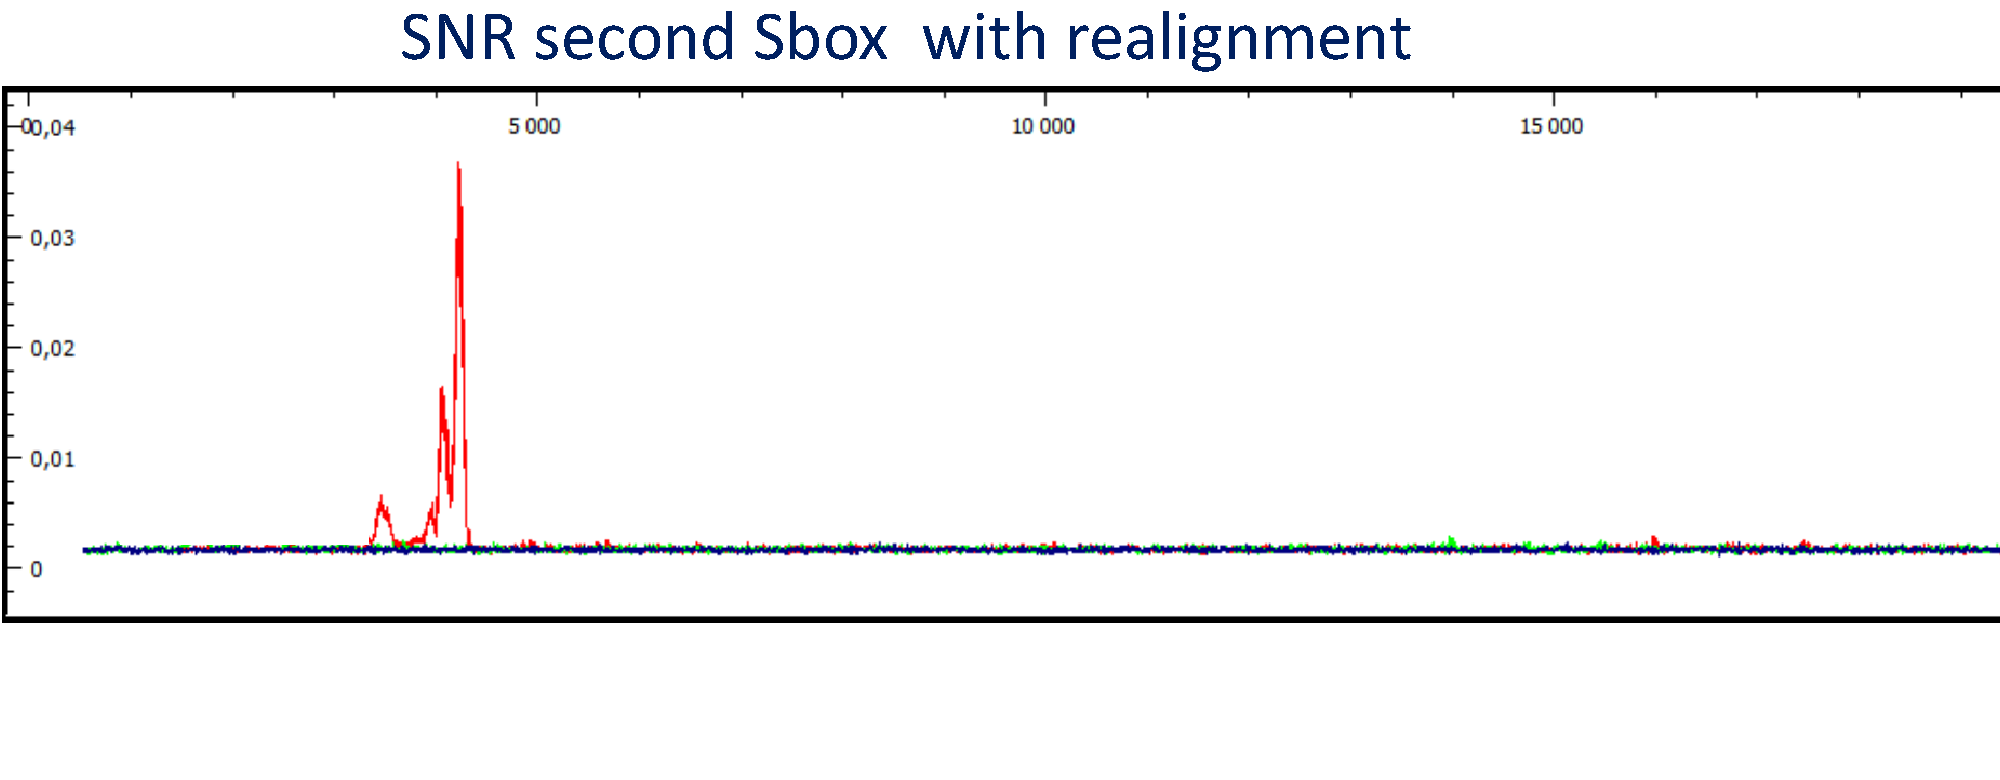
\includegraphics[width=0.75\textwidth]{../Figures/CHES2017/SNR_resynchro.pdf} 
}
\vspace*{-18pt}

\centering
\uncover<2>{
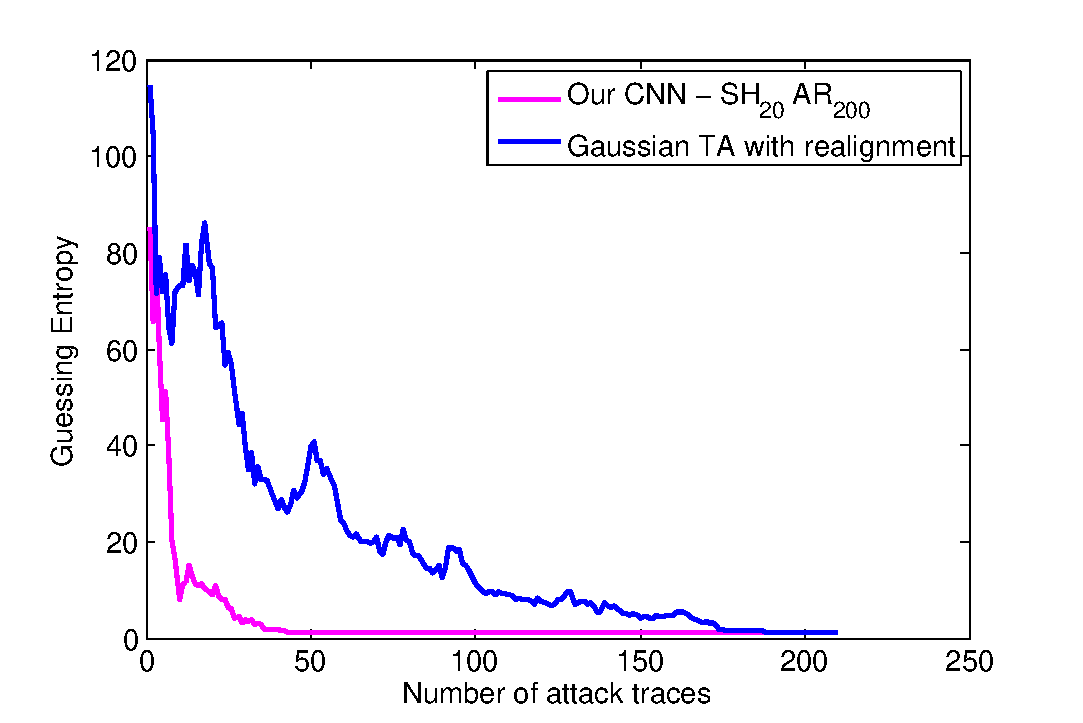
\includegraphics[width=0.5\textwidth]{../Figures/CHES2017/TA_CNN_smartcard.pdf} 
}


\end{frame}

%\begin{frame}\frametitle{Setup and Implementation}
%Target device and acquisitions: 
%
%\begin{itemize}
%\item 8-bit AVR microprocessor Atmega328P
%\item power-consumption acquired via the ChipWhisperer \cite{o2014chipwhisperer} platform
%\end{itemize}
%
%
%
%Implementation: 
%
%\begin{itemize}
%\item Begin of an AES-128
%\end{itemize}
%
%
%
%Attack: 
%
%
%\begin{itemize}
%\item Target sensitive variable: $Z = \mathrm{Sbox}(P_0 \oplus K_0)$
%\item Acquisition of $N_p\times 256$ profiling traces, under key knowledge
%\item Estimation of $C$-dimensional Gaussian templates via the projection of the profiling traces over the $C$ projecting components
%\item Template attack with $N$ attack traces
%\end{itemize}
%
%\end{frame}
%
%
%\begin{frame} \frametitle{The Problem of Selecting PCA Components - EGV}
%
%% state of the art
%% first and sixth PC DPA contest
%\begin{columns}
%\begin{column}{0.1\textwidth}
%\includegraphics[width = \textwidth]{figures/questionmark.jpg} 
%\end{column}
%\begin{column}{0.7\textwidth}
%\begin{block}{}
%{\em How many} PCs and {\em which ones} are sufficient/necessary to reduce the traces size without losing important discriminant information?
%\end{block}
%\end{column}
%\end{columns}
%\pause
%\begin{block}{Explained Global Variance (EGV)}
%$\EGV{\AAlpha_i} = \frac{\lambda_i}{\sum_{k=1}^r \lambda_k}$\\
%\cite{choudaryefficient} : 
%\begin{itemize}
%\item fix a threshold $\beta$
%\item choose the first $C$ components, where $C$ is the minimum integer such that
%\begin{equation*}
%\EGV{\AAlpha_1}+ \EGV{\AAlpha_2}+\dots + \EGV{\AAlpha_C} \geq \beta
%\end{equation*}
%\end{itemize}
%\end{block}
%
%
%
%\end{frame}
%
%
%\begin{frame} \frametitle{The Problem of Selecting PCA Components - Experimental Observation}
%\begin{block}{Experimental Observation}
%\cite{Batina2012,specht}: the first components sometimes contain more noise than information; it is worth discarding them.
%\end{block}
%\begin{figure}
%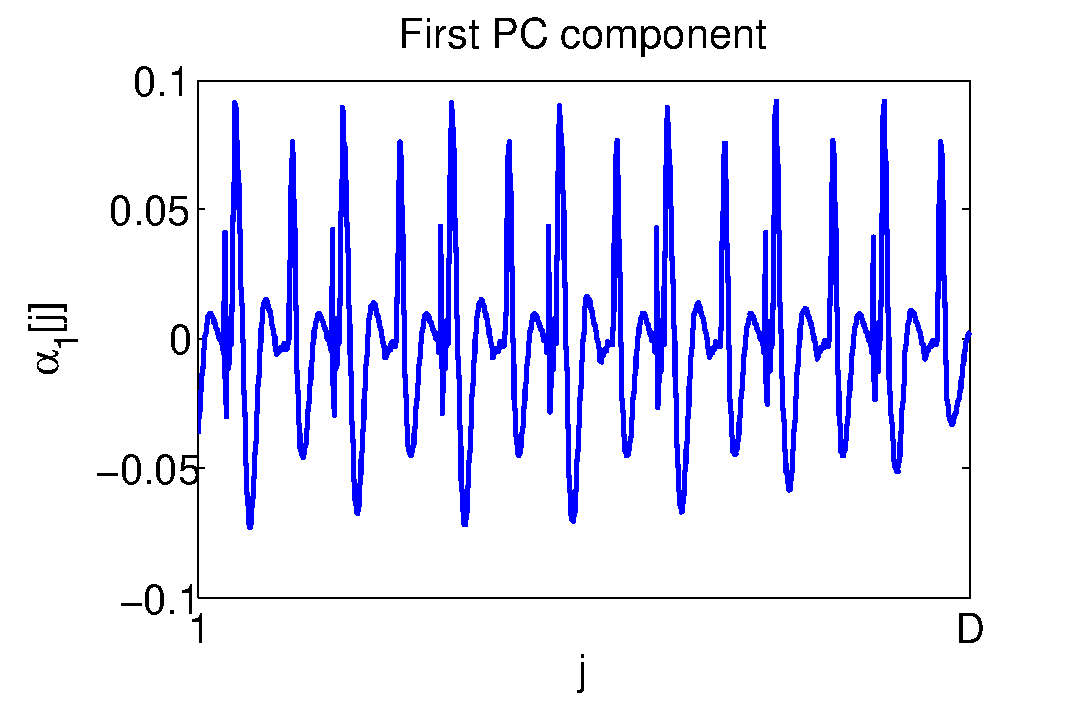
\includegraphics[width=.45\textwidth]{figures/DPAcontestPC1_new.pdf} 
%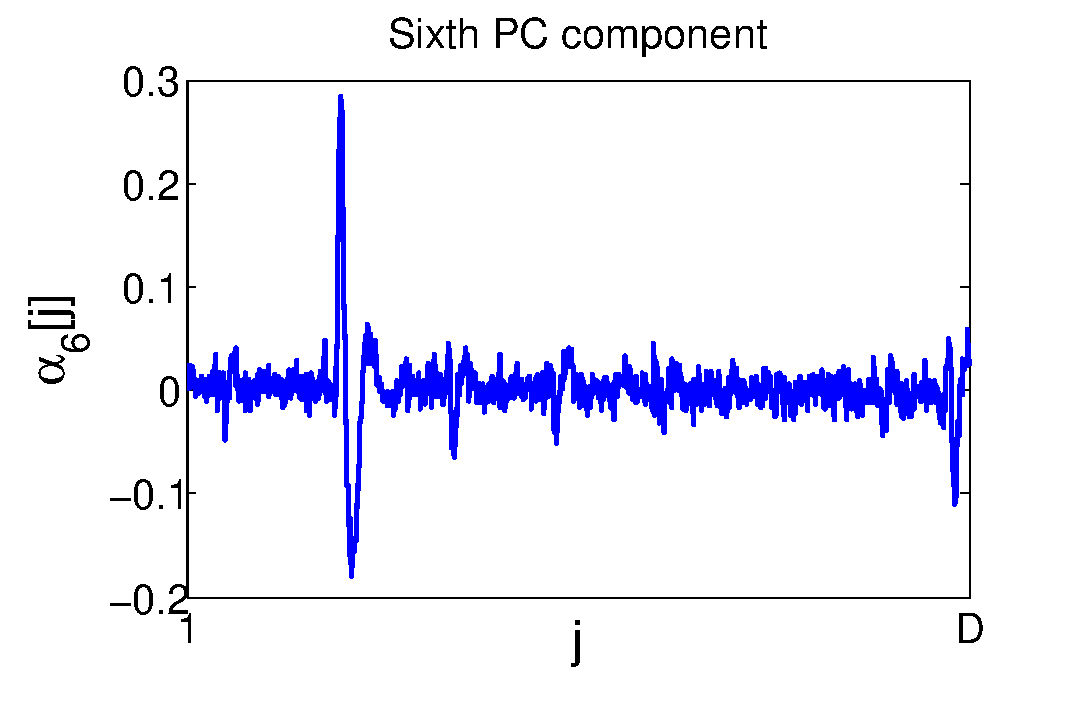
\includegraphics[width=.45\textwidth]{figures/DPAcontestPC6_new.pdf} 
%\caption{First and sixth PCs in DPA contest v4  \cite{DPAcontest} trace set}\label{fig:DPAcontest}
%\end{figure}
%\end{frame}
%
%\begin{frame} \frametitle{The Problem of Selecting PCA Components - IPR}
%\begin{block}{Assumption}
%Dealing with secured devices, the leaking side-channel information is localised in few points of the acquired trace.
%\end{block}
%\pause
%\begin{block}{Inverse Participation Ratio (IPR)}
%\cite{SCAclassProbl}: under the same assumption, use the IPR to choose informative components
%\begin{equation*}
%\mathrm{IPR}(\AAlpha_i) = \sum_{j=1}^\traceLength \AAlpha_i[j]^4 \mbox{ \em (localization score)}
%\end{equation*}
%\end{block}
%\end{frame}
%
%\begin{frame} \frametitle{The Explained Local Variance (ELV) Selection (1)}
%
%What minds to perform the choice of the PCs to keep:
%\begin{table}
%\begin{tabular}{|c|c|c|c|}
%\hline
%& EGV & IPR & \uncover<2->{\textbf{ELV}} \\
%\hline
%associated eigenvalue ($\lambda_i$) &
\includegraphics[scale=0.01]{figures/yes.png}  & 
\includegraphics[scale=0.01]{figures/no.png} &\uncover<2->{
\includegraphics[scale=0.015]{figures/yes.png}}\\
%\hline
%component form (localization of $\AAlpha_i$) &
\includegraphics[scale=0.01]{figures/no.png}  & 
\includegraphics[scale=0.01]{figures/yes.png}&\uncover<2->{
\includegraphics[scale=0.015]{figures/yes.png}} \\
%\hline
%\end{tabular}
%\end{table}
%
%\uncover<3->{
%\begin{block}{Inspection of $\lambda_i$}
%\begin{scriptsize}
%
%\begin{align*}
%\lambda_i =& \textcolor{gray}{\hat{\mathrm{var}}(\sum_{j=1}^D \XXX^\intercal[j]\AAlpha_i[j]) = \sum_{j=1}^D\sum_{k=1}^D \hat{\mathrm{cov}}(\XXX^\intercal[j]\AAlpha_i[j], \XXX^\intercal[k]\AAlpha_i[k])=}\\
%\textcolor{gray}{=}& \textcolor{gray}{\sum_{j=1}^D \AAlpha_i[j]\sum_{k=1}^D\AAlpha_i[k]\hat{\mathrm{cov}}(\XXX^\intercal[j], \XXX^\intercal[k])= \sum_{j=1}^D \AAlpha_i[j] (\covmat_{j}^\intercal \cdot \AAlpha_i)= } \\
%\textcolor{gray}{=}& \textcolor{gray}{\sum_{j=1}^D \AAlpha_i[j] \lambda_i\AAlpha_i[j] }= \sum_{j=1}^D  \lambda_i \AAlpha_i[j]^2 
%\end{align*}
%\end{scriptsize}
%
%The $j$-th time sample contribution to $\lambda_i$ is given by $\lambda_i \AAlpha_i[j]^2$
%\end{block}
%}
%
%
%\end{frame}
%
%\begin{frame} \frametitle{The ELV Selection (2)}
%\vspace*{-0.5cm}
%\uncover<1->{
%\begin{block}{Definition}
%$\mathrm{ELV}(\AAlpha_i,j) = \frac{\lambda_i \AAlpha_i[j]^2}{\sum_{k=1}^r\lambda_k} = \mathrm{EGV}(\AAlpha_i) \AAlpha_i[j]^2$  \\
%\uncover<2->{Observe that $\sum_{j=1}^D \mathrm{ELV}(\AAlpha_i,j) = \EGV{\AAlpha_i}$}
%\end{block}
%}
%\uncover<3->{
%Perform this sum in a cumulative way, sorting the ELV contributions of the time samples in decreasing order, {\em i. e.} $\mathrm{ELV}(\AAlpha_i,j^i_1)\geq \mathrm{ELV}(\AAlpha_i,j^i_2)\geq \dots \geq \mathrm{ELV}(\AAlpha_i,j^i_\traceLength)$
%
%
%\vspace*{-0.4cm}
%\begin{columns}
%\begin{column}{.5\textwidth}
%\vspace*{10pt}
%\begin{figure}
%\includegraphics[width=\textwidth]{figures/PC1_points.pdf} 
%\end{figure}
%\end{column}
%\begin{column}{.5\textwidth}
%\begin{figure}
%
%\begin{tikzpicture}[remember picture,
%    scale=1,
%    % Define styles here
%    every node/.style={transform shape}
%    block/.style={
%        rectangle,
%        draw,
%        text centered,
%        rounded corners
%        },
%    data/.style={
%        trapezium,
%        trapezium left angle=60,
%        trapezium right angle=120,
%        draw
%        },
%    component/.style={
%        circle,
%        draw
%        },
%    output/.style={
%        tape,
%        tape bend top=none,
%        draw
%        },
%    edge/.style={
%        ->,
%        >=stealth,
%        thick
%        }
%    ]
%
%    \node (only1elv) at (0,0)
%    {\includegraphics[width=\textwidth]{figures/cumulativeELV_only1.pdf} };
%    \node [component, thick, xshift=2.1cm, yshift=0.8cm] (cerchio) {};
%    \node[below left=1cm of cerchio](caption){$\mathrm{EGV}(\AAlpha_1)$};
%    \draw[->] (caption) to (cerchio.south west);
%\end{tikzpicture}
%\end{figure}
%\end{column}
%\end{columns}
%
%
%}
%
%\end{frame}
%
%
%
%\begin{frame}
%\frametitle{The ELV Selection (3)}
%\begin{columns}
%\begin{column}{0.5\textwidth}
%\uncover<1->{
%\only<1>{
%\vspace*{-0.4cm}
%\begin{center}
%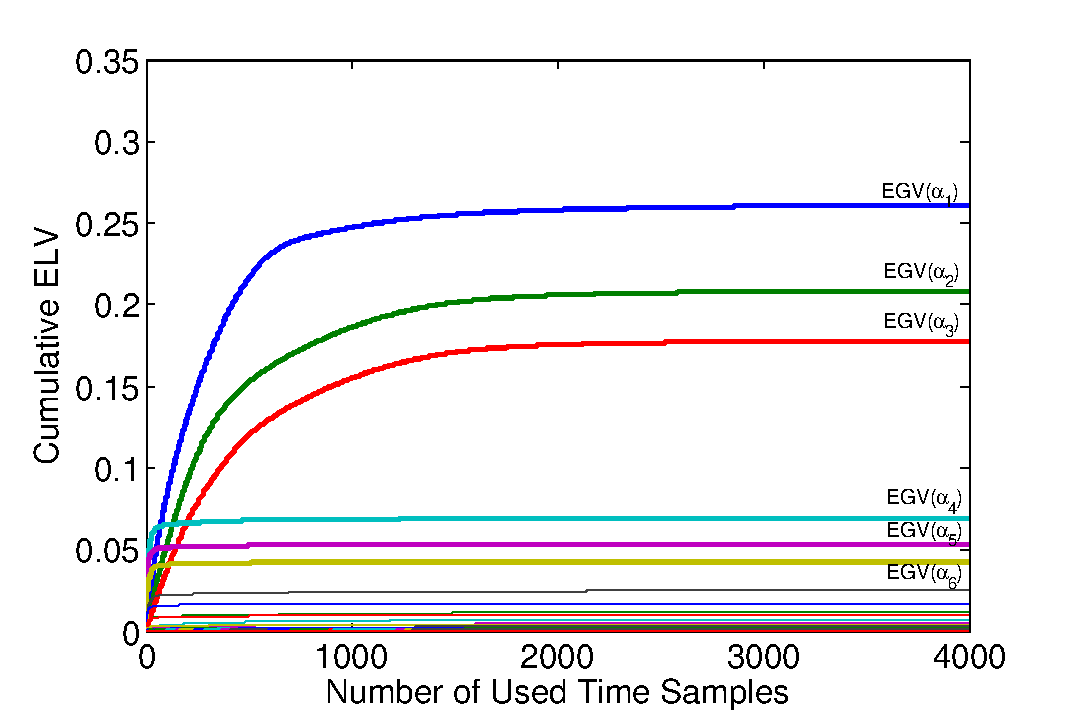
\includegraphics[width = \textwidth]{figures/cumulativeELV.pdf}
%\end{center}
%}
%\only<2>{
%\vspace*{-0.4cm}
%\begin{center}
%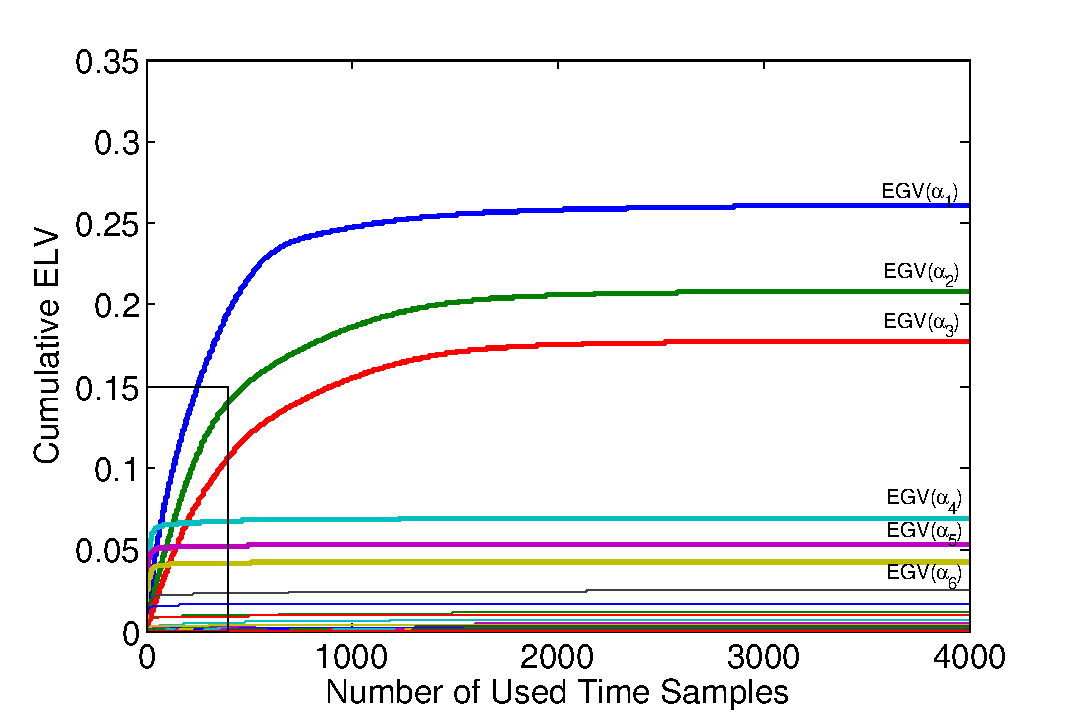
\includegraphics[width = \textwidth]{figures/cumulativeELVallRectangle.pdf} 
%\end{center}
%}
%
%\only<3->{
%\vspace*{-0.4cm}
%\begin{center}
%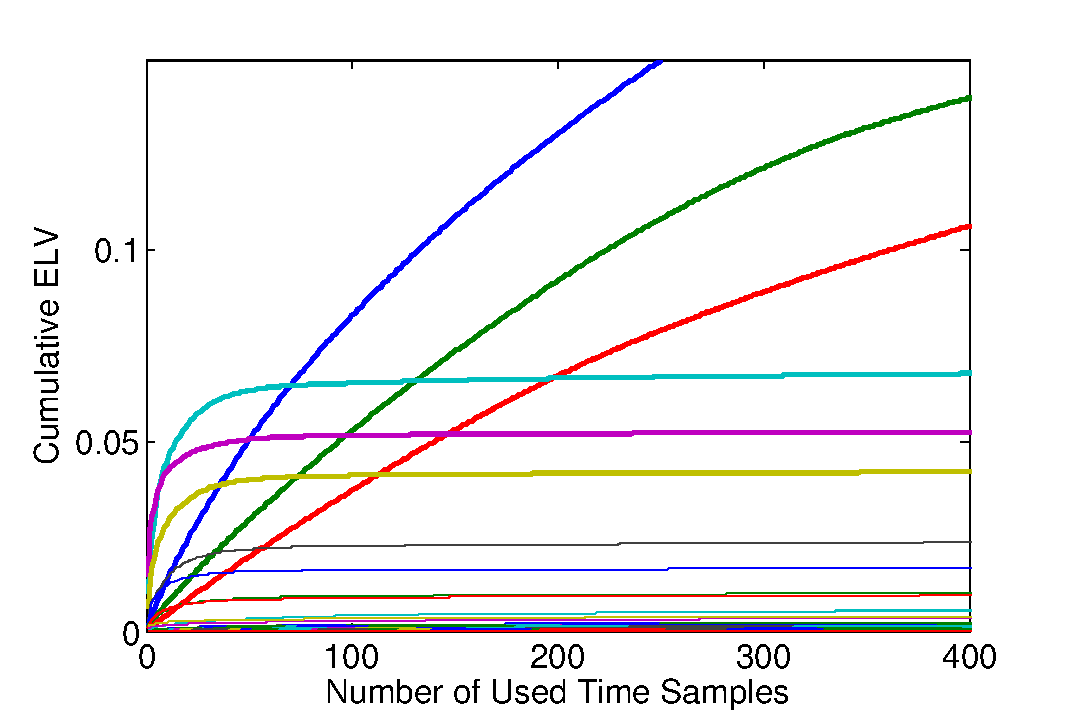
\includegraphics[width = \textwidth]{figures/cumulativeELVzoomed.pdf}
%\end{center}
%}
%}
%\uncover<4->{
%\only<1-4>{
%
%\begin{block}{To select $C$ components\hspace{\textwidth}\textcolor{white}{ }}
%Sort in decreasing order the maximal ELV provided by each component $\{\max_{j=1,\dots,D}\ELV(\AAlpha_i,j)\}_{i}$ and select the $C$ first components.
%\end{block}
%}
%\only<5>{
%
%\begin{block}{Fixing a cumulative explained variance threshold $\beta$}
%Select \textbf{couples} $(\AAlpha_i, j)$ in decreasing order wrt to $\ELV(\AAlpha_i, j)$ until $\ELV(\AAlpha_{i_1}, j_1)+ \ELV(\AAlpha_{i_2}, j_2)+\dots +\ELV(\AAlpha_{i_M}, j_M)\geq \beta$.\\
%%\uncover<5>{{\em Components denoising}}
%\end{block}
%}
%}
%
%\end{column}
%
%\begin{column}{0.5\textwidth}
%\only<1-3>{
%\begin{figure}
%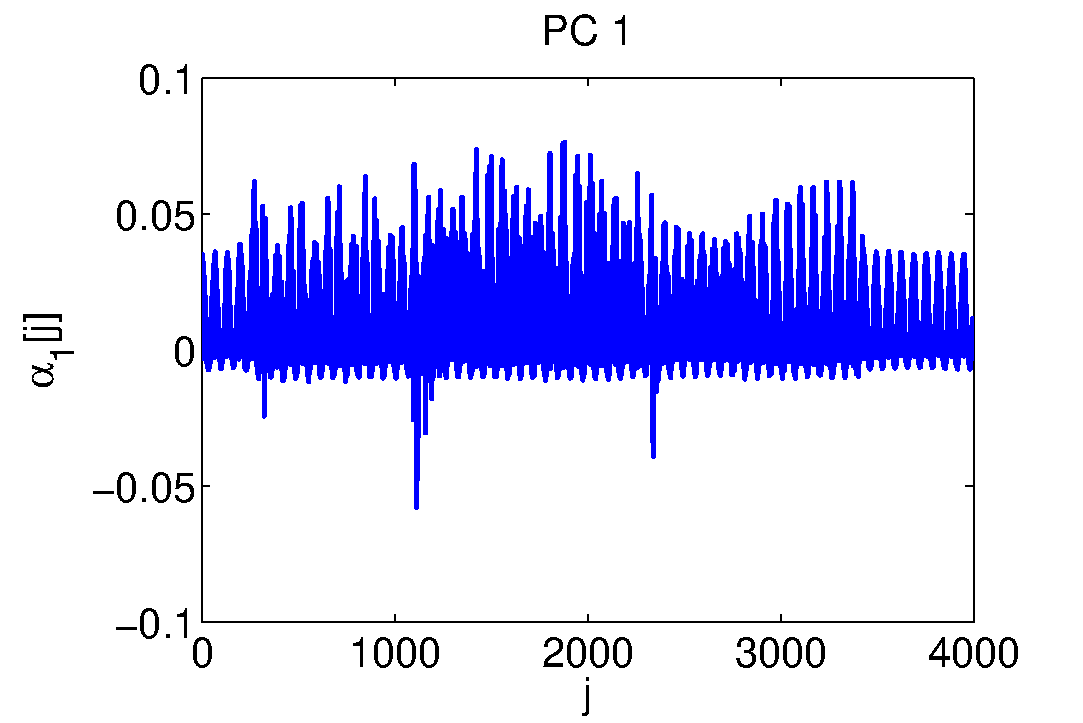
\includegraphics[width=0.5\textwidth]{figures/PC1.pdf} 
%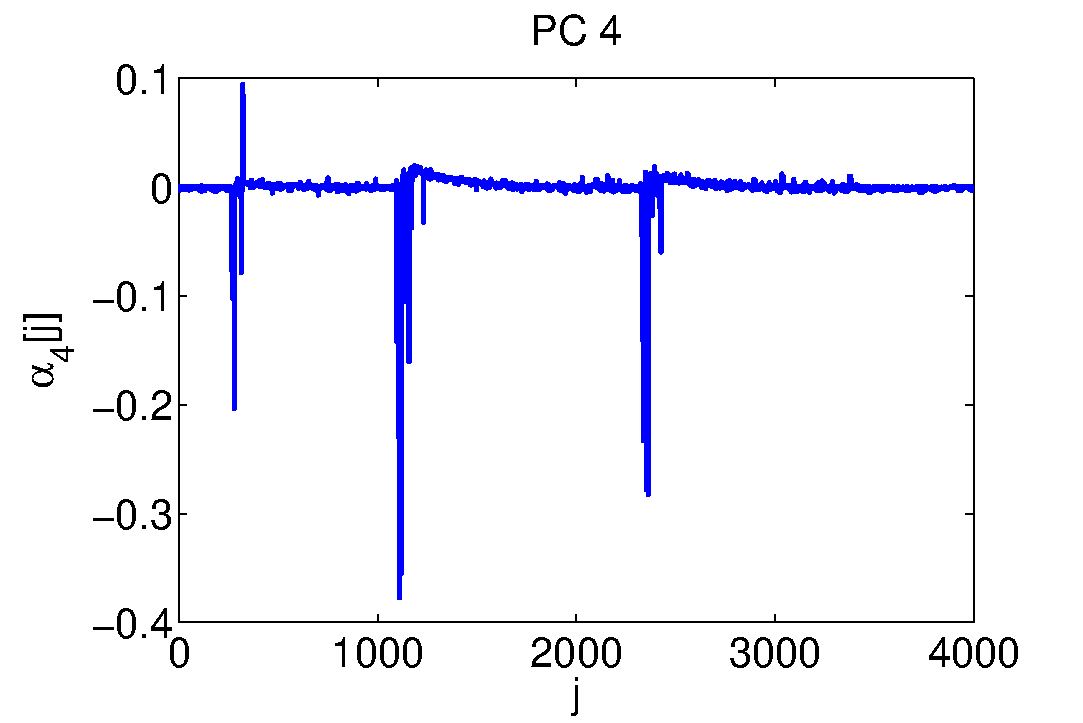
\includegraphics[width=0.5\textwidth]{figures/PC4.pdf} \\
%\includegraphics[width=0.5\textwidth]{figures/PC2.pdf} 
%\includegraphics[width=0.5\textwidth]{figures/PC5.pdf} \\
%\includegraphics[width=0.5\textwidth]{figures/PC3.pdf} 
%\includegraphics[width=0.5\textwidth]{figures/PC6.pdf} 
%\caption{\begin{footnotesize}
%The first 6 PCs: 
%$\lambda_1 \approx 3.8 ,\lambda_2 \approx 3.1 , \lambda_3 \approx2.6 ,\lambda_4 \approx 1.0 ,\lambda_5 \approx 0.8 ,\lambda_6 \approx 0.6 $
%\end{footnotesize}}
%
%\end{figure}
%}
%
%
%\only<4-5>{
%\begin{figure}
%\onslide<5->{\includegraphics[width=0.5\textwidth]{figures/PC5_denoised.pdf}}\only<4>{\includegraphics[width=0.5\textwidth]{figures/PC5_cerchio.pdf}}\only<5>{\includegraphics[width=0.5\textwidth]{figures/PC5_cerchio_transp.pdf}} \\
%\onslide<5->{\includegraphics[width=0.5\textwidth]{figures/PC4_denoised.pdf}}\only<4>{\includegraphics[width=0.5\textwidth]{figures/PC4_cerchio.pdf}}\only<5>{\includegraphics[width=0.5\textwidth]{figures/PC4_cerchio_transp.pdf}} \\
%\onslide<5->{\includegraphics[width=0.5\textwidth]{figures/PC6_denoised.pdf}}\only<4>{\includegraphics[width=0.5\textwidth]{figures/PC6_cerchio.pdf}}\only<5>{\includegraphics[width=0.5\textwidth]{figures/PC6_cerchio_transp.pdf}} 
%\only<4>{\caption{The 3 components chosen by ELV selection method - $C$ fixed}}
%\only<5>{\caption{Components and time samples chosen by ELV selection method - $\beta$ fixed}}
%\end{figure}
%}
%
%
%%\only<5>{
%%\includegraphics[width=0.31\textwidth]{ figures/PC5_cerchio_transp.pdf} 
%%\includegraphics[width=0.31\textwidth]{ figures/PC4_cerchio_transp.pdf} 
%%\includegraphics[width=0.31\textwidth]{ figures/PC6_cerchio_transp.pdf} \\
%%}
%%\uncover<5>{
%%
%%
%%
%%\only<3-4>{\caption{Selected components for $C = 3$; \hspace{\textwidth} $\ELV(\AAlpha_5, 2362)\approx 0.41$, $\ELV(\AAlpha_4, 1110)\approx 0.38$, $\ELV(\AAlpha_6, 1118)\approx 0.24$}}
%%\only<5>{\caption{Selected and denoised components for $\beta = 0.08$\hspace{\textwidth}\textcolor{white}{$\ELV(\AAlpha_5, 2362)\approx 0.41$, $\ELV(\AAlpha_4, 1110)\approx 0.38$, $\ELV(\AAlpha_6, 1118)\approx 0.24$}}}
%
%\end{column}
%
%\end{columns}
%
%
%\end{frame}
%
%%\begin{frame} \frametitle{The Component Selection Issue}
%%
%%\begin{columns}
%%\begin{column}{0.1\textwidth}
%%\includegraphics[width = \textwidth]{figures/questionmark.jpg} 
%%\end{column}
%%\begin{column}{0.7\textwidth}
%%\begin{block}{}
%%{\em How many} PCs and {\em which ones} are sufficient/necessary to reduce the traces size without losing important discriminant information? 
%%\end{block}
%%\end{column}
%%\end{columns}
%% \only<1>{
%% \begin{block}{Theoretically}
%%Higher eigenvalues $\longrightarrow$ higher information.
%%\end{block}
%%\begin{block}{Experimental Observation}
%%\cite{Batina2012,specht}: the first components sometimes contain no sensitive information; it is worth discarding them.
%%\end{block}
%%
%%\begin{figure}
%%\includegraphics[width=.25\textwidth]{figures/DPAcontestPC1_new.pdf} 
%%\includegraphics[width=.25\textwidth]{figures/DPAcontestPC6_new.pdf} 
%%\vspace{-10pt}
%%\caption{First and sixth PCs in DPA contest v4  \cite{DPAcontest} trace set}\label{fig:DPAcontest}
%%\end{figure}
%%}
%%\only<2>{
%%\vspace{40pt}
%%\begin{small}
%%\begin{table}
%%\begin{tabular}{|c|c|c|c|}
%%\hline
%%& EGV \cite{choudaryefficient} & IPR \cite{SCAclassProbl}& \uncover<2->{\textbf{ELV} \cite{Cagli2016}} \\
%%\hline
%%eigenvalue $\lambda_i$ &\includegraphics[scale=0.01]{figures/yes.png}  & \includegraphics[scale=0.01]{figures/no.png} &\uncover<2->{\includegraphics[scale=0.015]{figures/yes.png}}\\
%%\hline
%%form of $\AAlpha_i$ &\includegraphics[scale=0.01]{figures/no.png}  & \includegraphics[scale=0.01]{figures/yes.png}&\uncover<2->{\includegraphics[scale=0.015]{figures/yes.png}} \\
%%\hline
%%\end{tabular}
%%\end{table}
%%\end{small}
%%
%%\includegraphics[scale=0.3]{figures/citazione1.jpg} 
%%}
%%\uncover<2->{
%%\begin{block}{Explained Local Variance}
%%$\mathrm{ELV}(\AAlpha_i,j) = \frac{\lambda_i \AAlpha_i[j]^2}{\sum_{k=1}^r\lambda_k} = \mathrm{EGV}(\AAlpha_i) \AAlpha_i[j]^2$  \\
%%%($\sum_{j=1}^D \mathrm{ELV}(\AAlpha_i,j) = \EGV{\AAlpha_i}$)
%%\end{block}
%%}
%%\uncover<3->{\begin{block}{Use of the ELV}
%%\begin{itemize}
%%\item Sort in decreasing order the maximal ELV provided by each component $\{\max_{j=1,\dots,D}\ELV(\AAlpha_i,j)\}_{i}$ and select the $C$ first components.
%%\item Select \textbf{couples} $(\AAlpha_i, j)$ in decreasing order wrt to $\ELV(\AAlpha_i, j)$ until $\ELV(\AAlpha_{i_1}, j_1)+ \ELV(\AAlpha_{i_2}, j_2)+\dots +\ELV(\AAlpha_{i_M}, j_M)\geq \beta$
%%\end{itemize}
%%\end{block}}
%%\end{frame}
%%
%%\begin{frame} \frametitle{The ELV Selection (2)}
%%\vspace*{-0.5cm}
%%\uncover<1->{
%%\begin{block}{Definition}
%%$\mathrm{ELV}(\AAlpha_i,j) = \frac{\lambda_i \AAlpha_i[j]^2}{\sum_{k=1}^r\lambda_k} = \mathrm{EGV}(\AAlpha_i) \AAlpha_i[j]^2$  \\
%%\uncover<2->{Observe that $\sum_{j=1}^D \mathrm{ELV}(\AAlpha_i,j) = \EGV{\AAlpha_i}$}
%%\end{block}
%%}
%%\uncover<3->{
%%Perform this sum in a cumulative way, sorting the ELV contributions of the time samples in decreasing order, {\em i. e.} $\mathrm{ELV}(\AAlpha_i,j^i_1)\geq \mathrm{ELV}(\AAlpha_i,j^i_2)\geq \dots \geq \mathrm{ELV}(\AAlpha_i,j^i_\traceLength)$
%%
%%
%%\vspace*{-0.4cm}
%%\begin{columns}
%%\begin{column}{.5\textwidth}
%%\vspace*{10pt}
%%\begin{figure}
%%\includegraphics[width=\textwidth]{figures/PC1_points.pdf} 
%%\end{figure}
%%\end{column}
%%\begin{column}{.5\textwidth}
%%\begin{figure}
%%
%%\begin{tikzpicture}[remember picture,
%%    scale=1,
%%    % Define styles here
%%    every node/.style={transform shape}
%%    block/.style={
%%        rectangle,
%%        draw,
%%        text centered,
%%        rounded corners
%%        },
%%    data/.style={
%%        trapezium,
%%        trapezium left angle=60,
%%        trapezium right angle=120,
%%        draw
%%        },
%%    component/.style={
%%        circle,
%%        draw
%%        },
%%    output/.style={
%%        tape,
%%        tape bend top=none,
%%        draw
%%        },
%%    edge/.style={
%%        ->,
%%        >=stealth,
%%        thick
%%        }
%%    ]
%%
%%    \node (only1elv) at (0,0)
%%    {\includegraphics[width=\textwidth]{figures/cumulativeELV_only1.pdf} };
%%    \node [component, thick, xshift=2.1cm, yshift=0.8cm] (cerchio) {};
%%    \node[below left=1cm of cerchio](caption){$\mathrm{EGV}(\AAlpha_1)$};
%%    \draw[->] (caption) to (cerchio.south west);
%%\end{tikzpicture}
%%\end{figure}
%%\end{column}
%%\end{columns}
%%
%%
%%}
%%
%%\end{frame}
%%
%%
%%
%%%\begin{frame}
%%\frametitle{The ELV Selection (2)}
%%\begin{columns}
%%\begin{column}{0.5\textwidth}
%%\uncover<1->{
%%\only<1>{
%%\vspace*{-0.4cm}
%%\begin{center}
%%\includegraphics[width = \textwidth]{figures/cumulativeELV.pdf}
%%\end{center}
%%}
%%\only<2>{
%%\vspace*{-0.4cm}
%%\begin{center}
%%\includegraphics[width = \textwidth]{figures/cumulativeELVallRectangle.pdf} 
%%\end{center}
%%}
%%
%%\only<3->{
%%\vspace*{-0.4cm}
%%\begin{center}
%%\includegraphics[width = \textwidth]{figures/cumulativeELVzoomed.pdf}
%%\end{center}
%%}
%%}
%%\uncover<4->{
%%\only<1-4>{
%%
%%\begin{block}{To select $C$ components\hspace{\textwidth}\textcolor{white}{ }}
%%Sort in decreasing order the maximal ELV provided by each component $\{\max_{j=1,\dots,D}\ELV(\AAlpha_i,j)\}_{i}$ and select the $C$ first components.
%%\end{block}
%%}
%%\only<5>{
%%
%%\begin{block}{Fixing a cumulative explained variance threshold $\beta$}
%%Select \textbf{couples} $(\AAlpha_i, j)$ in decreasing order wrt to $\ELV(\AAlpha_i, j)$ until $\ELV(\AAlpha_{i_1}, j_1)+ \ELV(\AAlpha_{i_2}, j_2)+\dots +\ELV(\AAlpha_{i_M}, j_M)\geq \beta$.\\
%%%\uncover<5>{{\em Components denoising}}
%%\end{block}
%%}
%%}
%%
%%\end{column}
%%
%%\begin{column}{0.5\textwidth}
%%\only<1-3>{
%%\begin{figure}
%%\includegraphics[width=0.5\textwidth]{figures/PC1.pdf} 
%%\includegraphics[width=0.5\textwidth]{figures/PC4.pdf} \\
%%\includegraphics[width=0.5\textwidth]{figures/PC2.pdf} 
%%\includegraphics[width=0.5\textwidth]{figures/PC5.pdf} \\
%%\includegraphics[width=0.5\textwidth]{figures/PC3.pdf} 
%%\includegraphics[width=0.5\textwidth]{figures/PC6.pdf} 
%%\caption{\begin{footnotesize}
%%The first 6 PCs: 
%%$\lambda_1 \approx 3.8 ,\lambda_2 \approx 3.1 , \lambda_3 \approx2.6 ,\lambda_4 \approx 1.0 ,\lambda_5 \approx 0.8 ,\lambda_6 \approx 0.6 $
%%\end{footnotesize}}
%%
%%\end{figure}
%%}
%%
%%
%%\only<4-5>{
%%\begin{figure}
%%\onslide<5->{\includegraphics[width=0.5\textwidth]{figures/PC5_denoised.pdf}}\only<4>{\includegraphics[width=0.5\textwidth]{figures/PC5_cerchio.pdf}}\only<5>{\includegraphics[width=0.5\textwidth]{figures/PC5_cerchio_transp.pdf}} \\
%%\onslide<5->{\includegraphics[width=0.5\textwidth]{figures/PC4_denoised.pdf}}\only<4>{\includegraphics[width=0.5\textwidth]{figures/PC4_cerchio.pdf}}\only<5>{\includegraphics[width=0.5\textwidth]{figures/PC4_cerchio_transp.pdf}} \\
%%\onslide<5->{\includegraphics[width=0.5\textwidth]{figures/PC6_denoised.pdf}}\only<4>{\includegraphics[width=0.5\textwidth]{figures/PC6_cerchio.pdf}}\only<5>{\includegraphics[width=0.5\textwidth]{figures/PC6_cerchio_transp.pdf}} 
%%\only<4>{\caption{The 3 components chosen by ELV selection method - $C$ fixed}}
%%\only<5>{\caption{Components and time samples chosen by ELV selection method - $\beta$ fixed}}
%%\end{figure}
%%}
%%
%%
%%\only<5>{
%%\includegraphics[width=0.31\textwidth]{figures/PC5_cerchio_transp.pdf} 
%%\includegraphics[width=0.31\textwidth]{figures/PC4_cerchio_transp.pdf} 
%%\includegraphics[width=0.31\textwidth]{figures/PC6_cerchio_transp.pdf} \\
%%}
%%\uncover<5>{
%%
%%
%%
%%\only<3-4>{\caption{Selected components for $C = 3$; \hspace{\textwidth} $\ELV(\AAlpha_5, 2362)\approx 0.41$, $\ELV(\AAlpha_4, 1110)\approx 0.38$, $\ELV(\AAlpha_6, 1118)\approx 0.24$}}
%%\only<5>{\caption{Selected and denoised components for $\beta = 0.08$\hspace{\textwidth}\textcolor{white}{$\ELV(\AAlpha_5, 2362)\approx 0.41$, $\ELV(\AAlpha_4, 1110)\approx 0.38$, $\ELV(\AAlpha_6, 1118)\approx 0.24$}}}
%%
%%\end{column}
%%
%%\end{columns}
%%
%%
%%\end{frame}
%%